\chapter{Results} \label{chap:results}

  \newcommand\plotwidth{0.95\textwidth}
  \newcommand\imagewidth{0.40\textwidth}
  	
  \begin{notes}
    \item Write chapter introduction	
  \end{notes}

  \section{Terrains} % Before and After
  
    \begin{notes}
      \item Show some comparison between base surfaces and results with different parameters.
    \end{notes}
  
	\begin{figure}[H]
		\centering
		
\includegraphics[width=\imagewidth]{images/results/terrains/512-1/orig}
		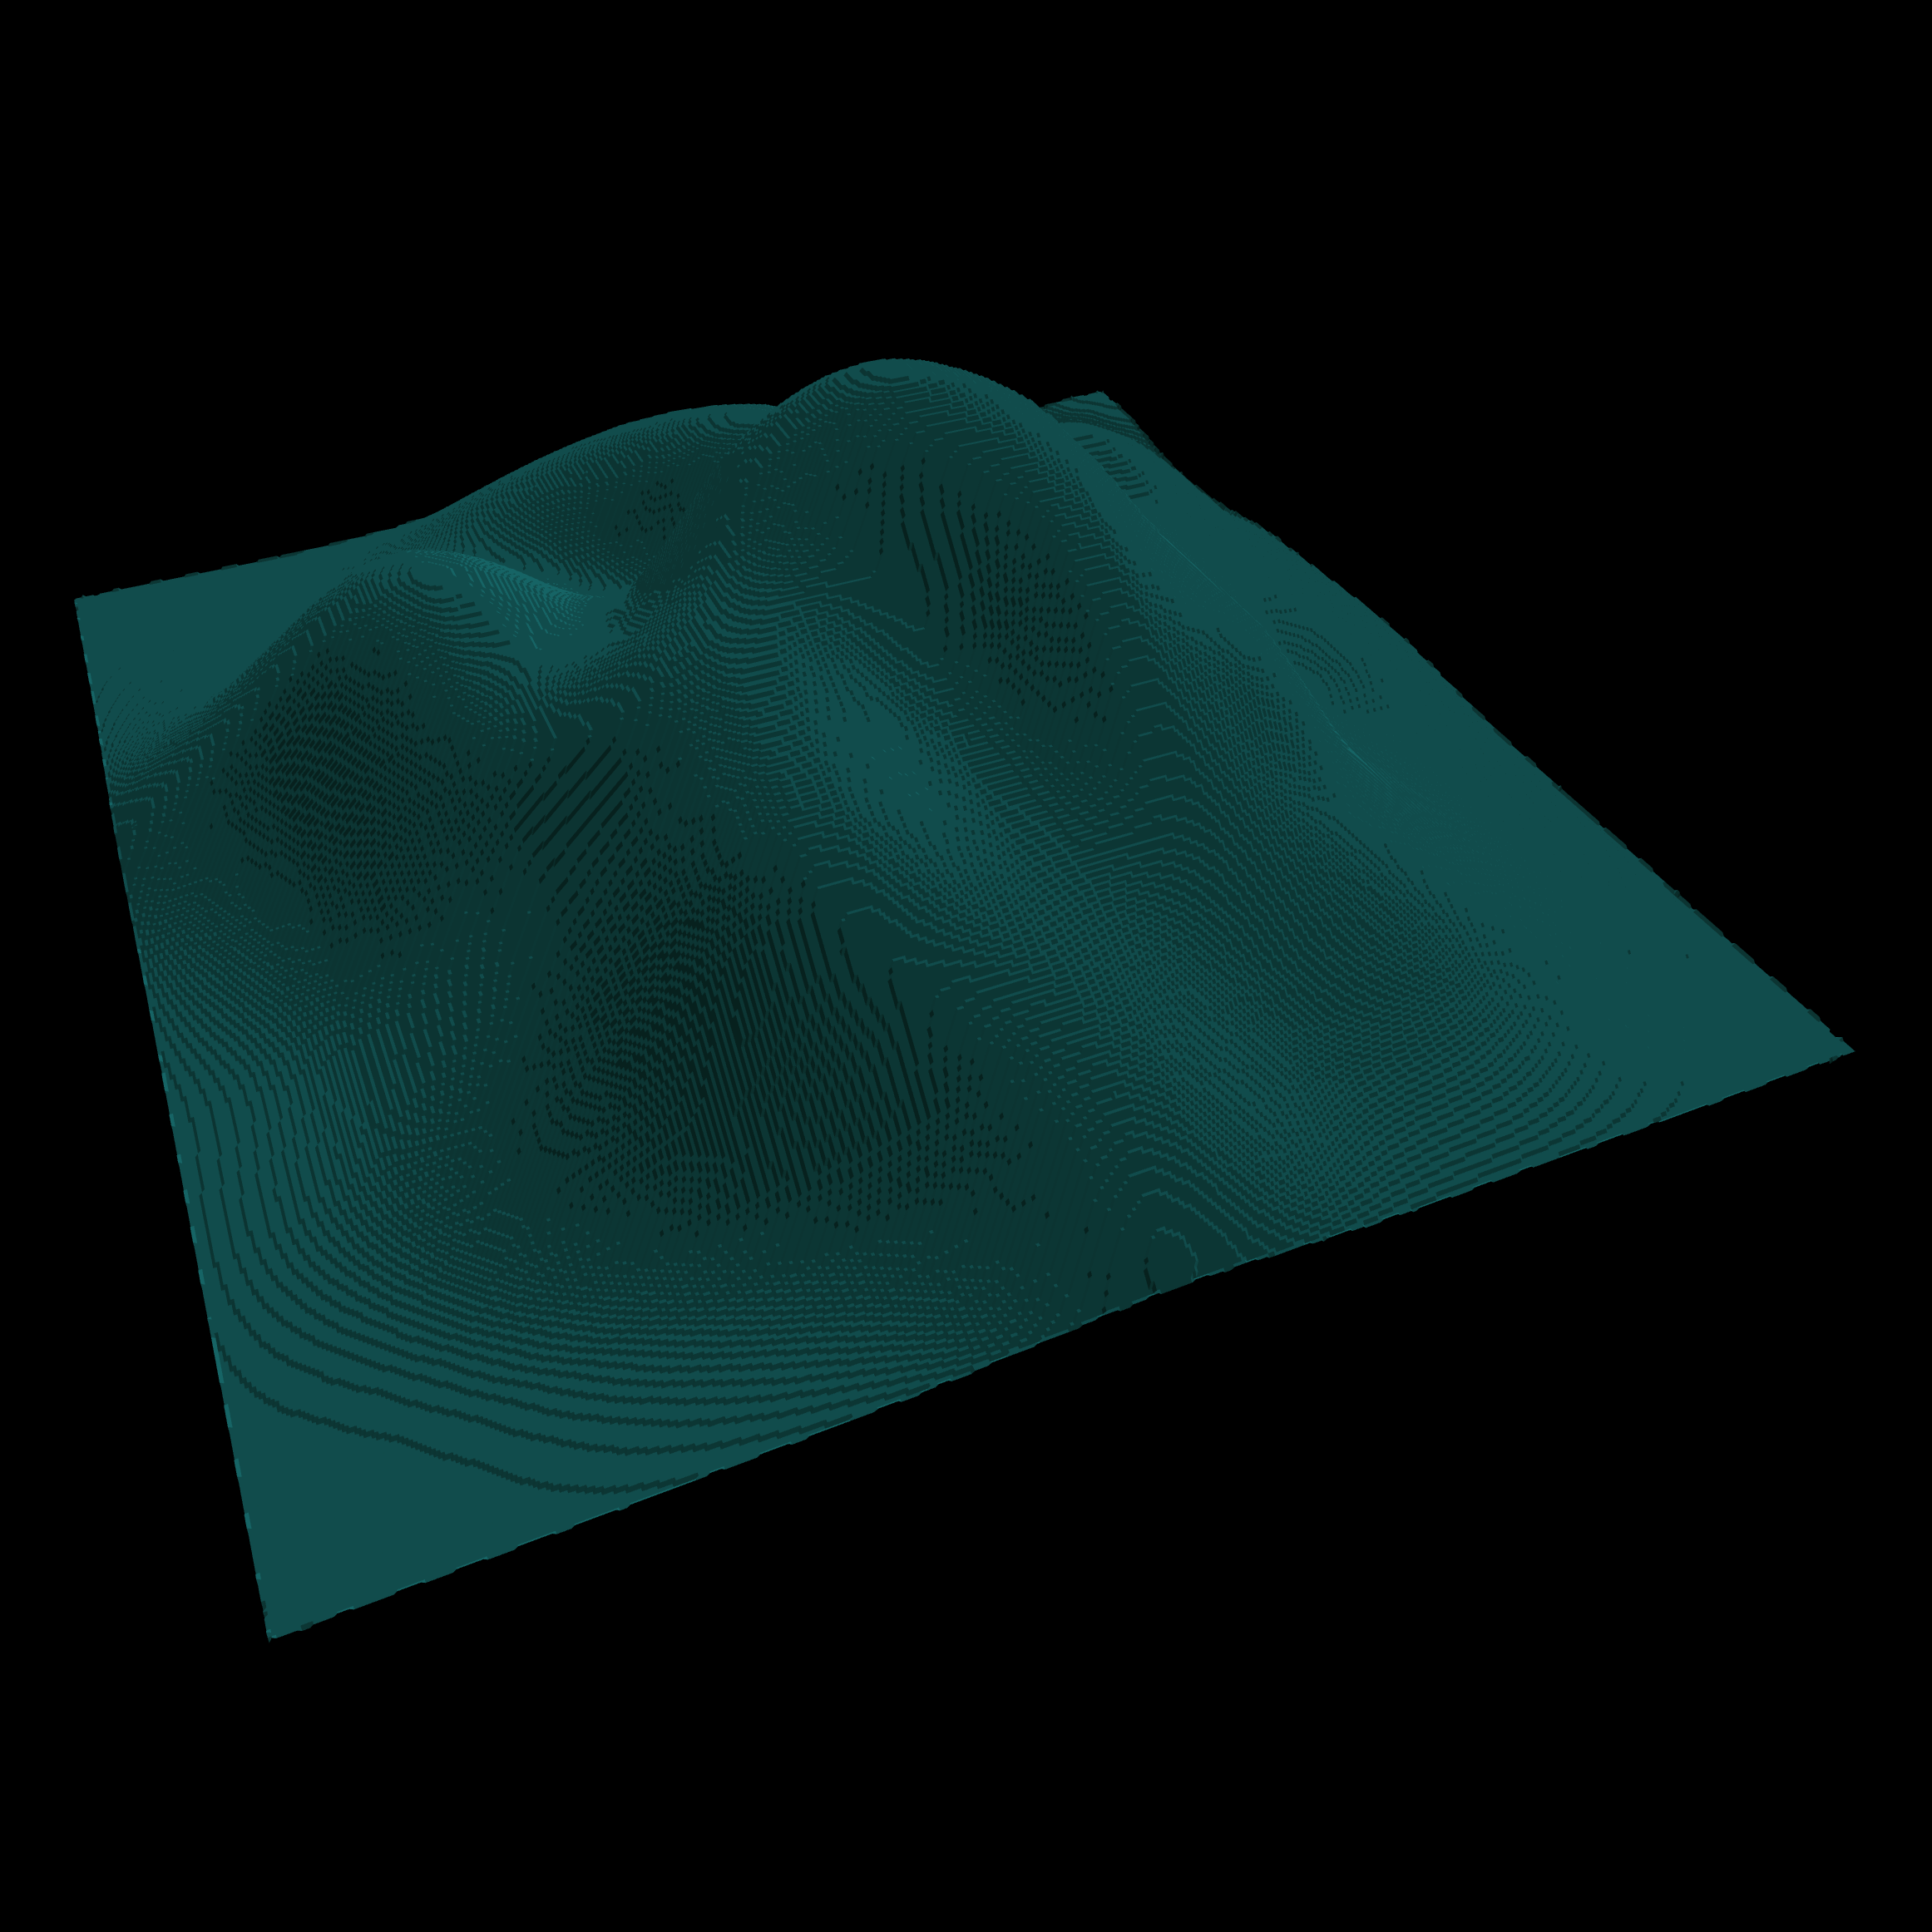
\includegraphics[width=\imagewidth]{images/results/terrains/512-1/orig_3d}
		\caption{Base surface used in the examples}
		\label{fig:ex-base-surface}
	\end{figure}
  
    \subsection {Fourier Filtering Generation}
		
		\begin{figure}[H]
		  \centering
		  
\includegraphics[width=\imagewidth]{images/results/terrains/512-1/fourier/18}
		  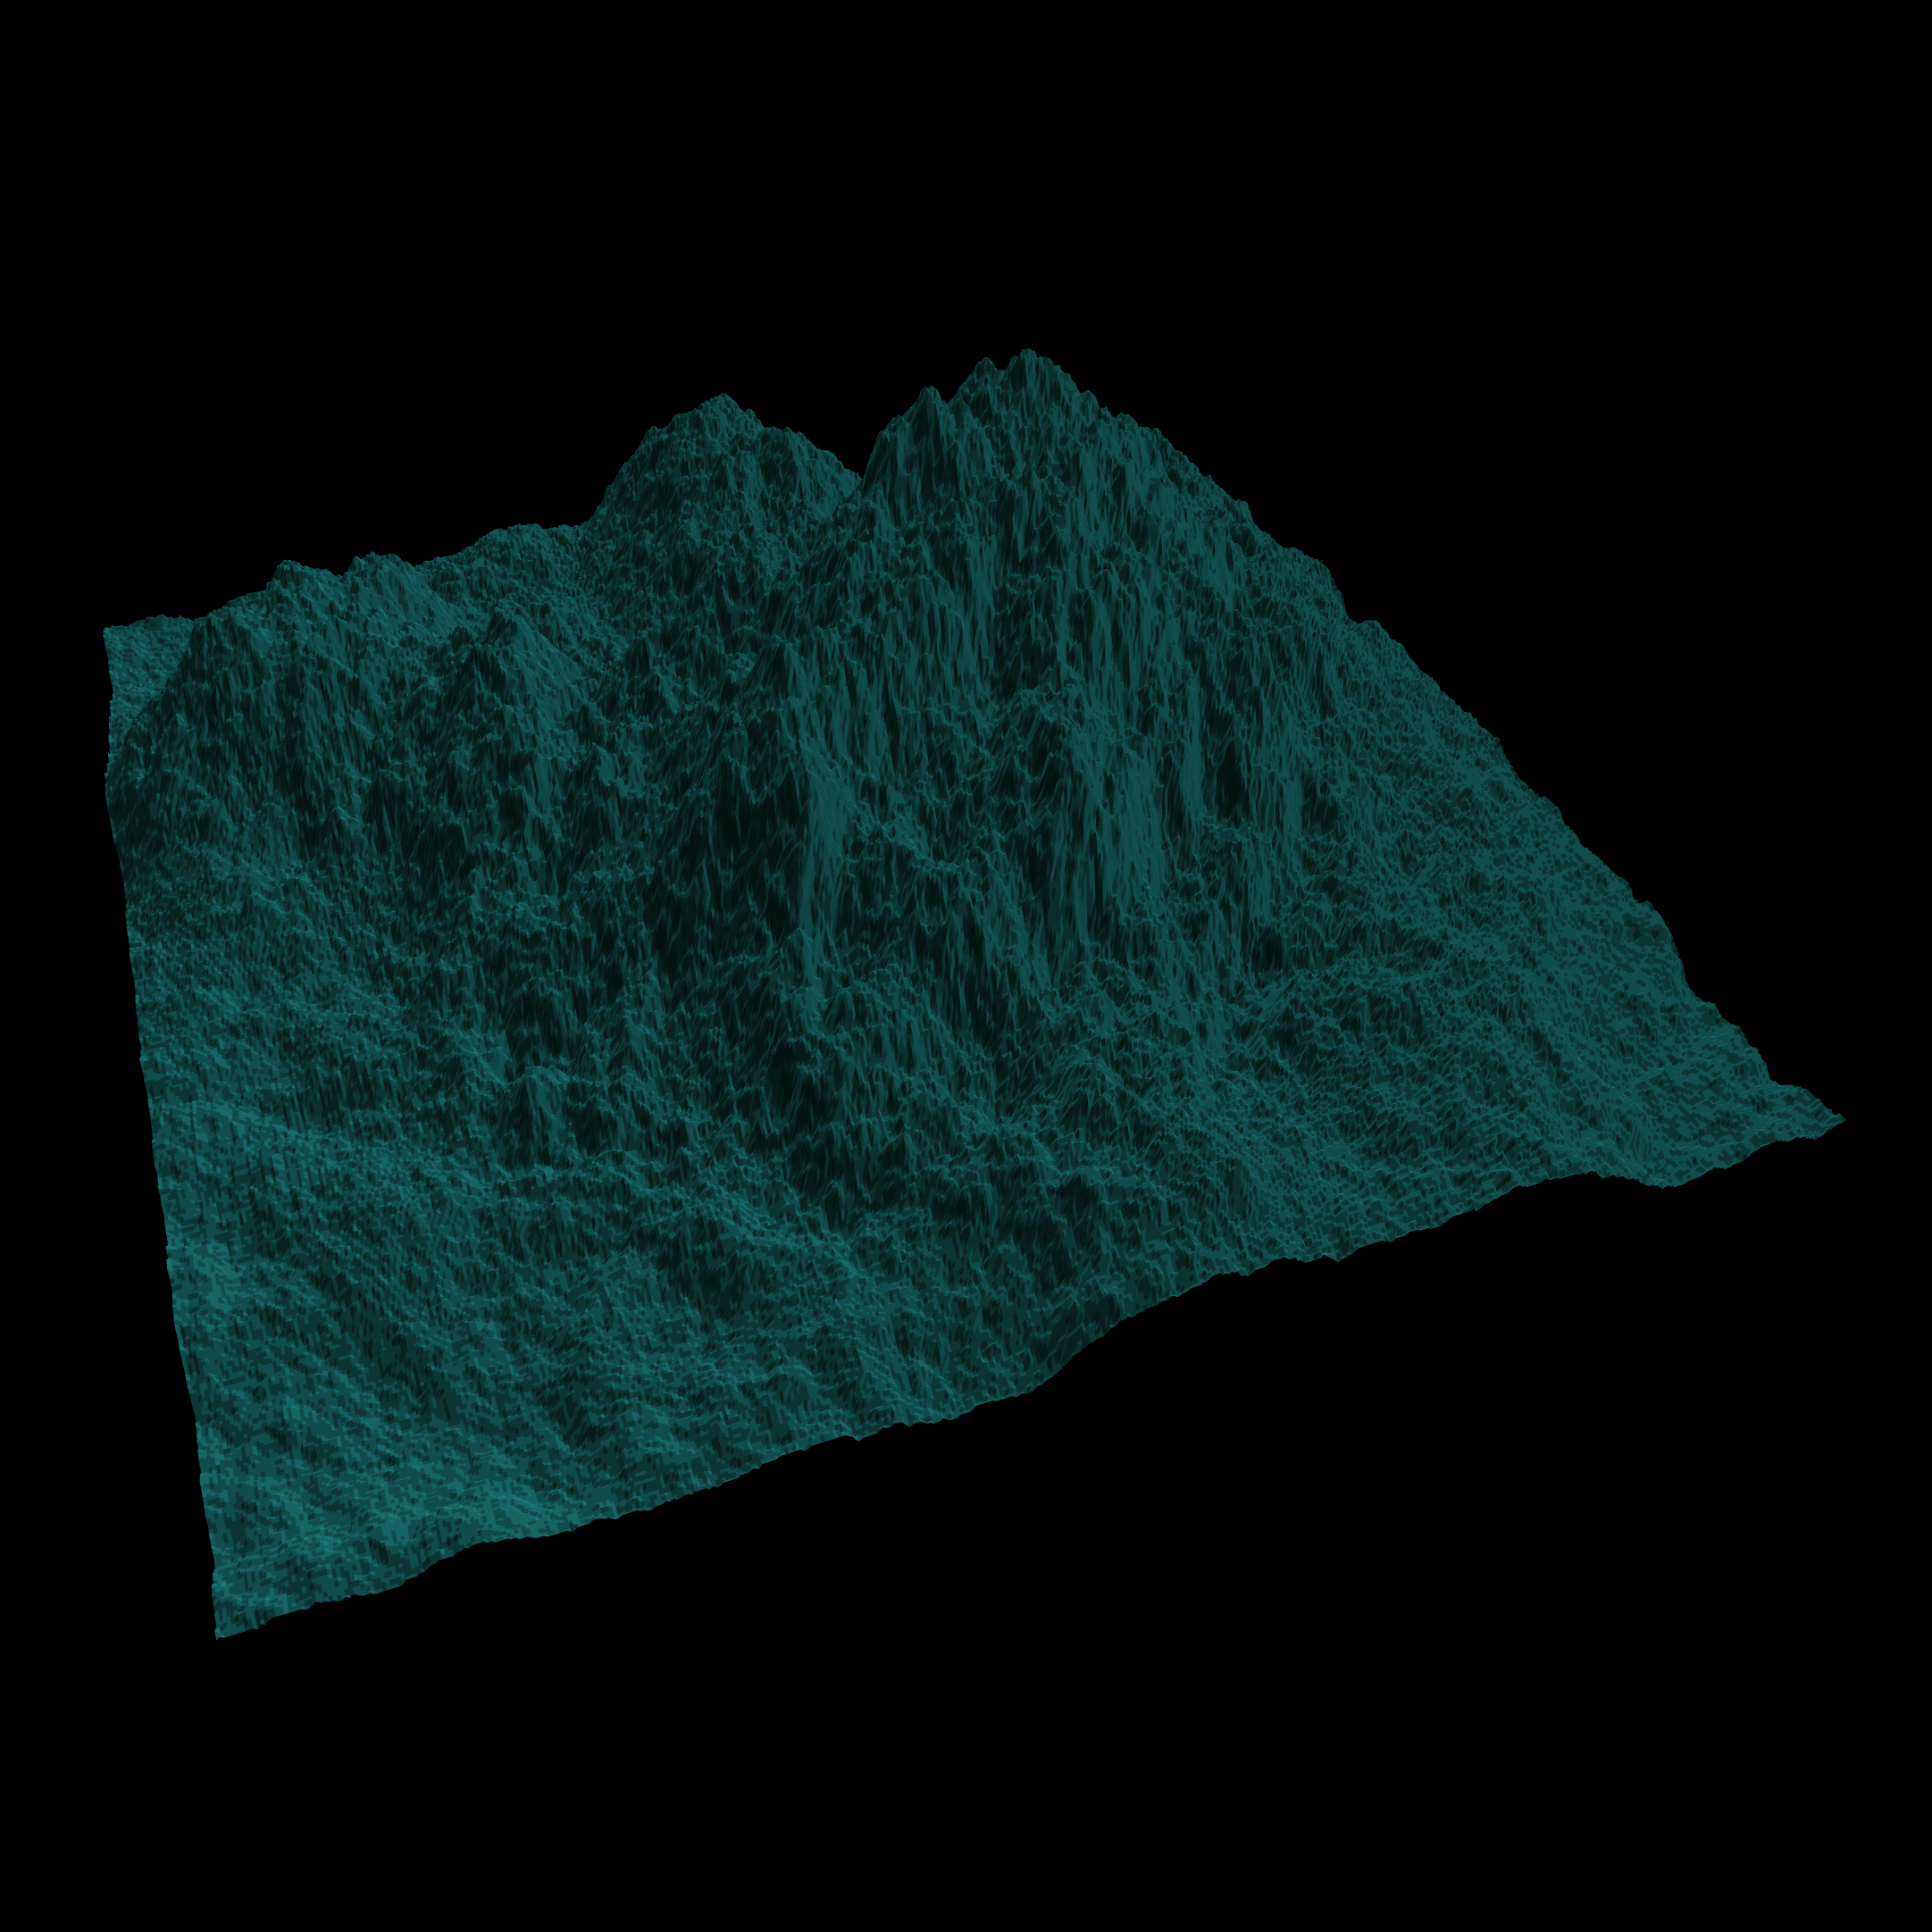
\includegraphics[width=\imagewidth]{images/results/terrains/512-1/fourier/18_3d}
		  \caption{$\beta = 1.8$}
		  \label{fig:ex-fourier18-surface}
		\end{figure}
		
		\begin{figure}[H]
		  \centering
		  
\includegraphics[width=\imagewidth]{images/results/terrains/512-1/fourier/20}
		  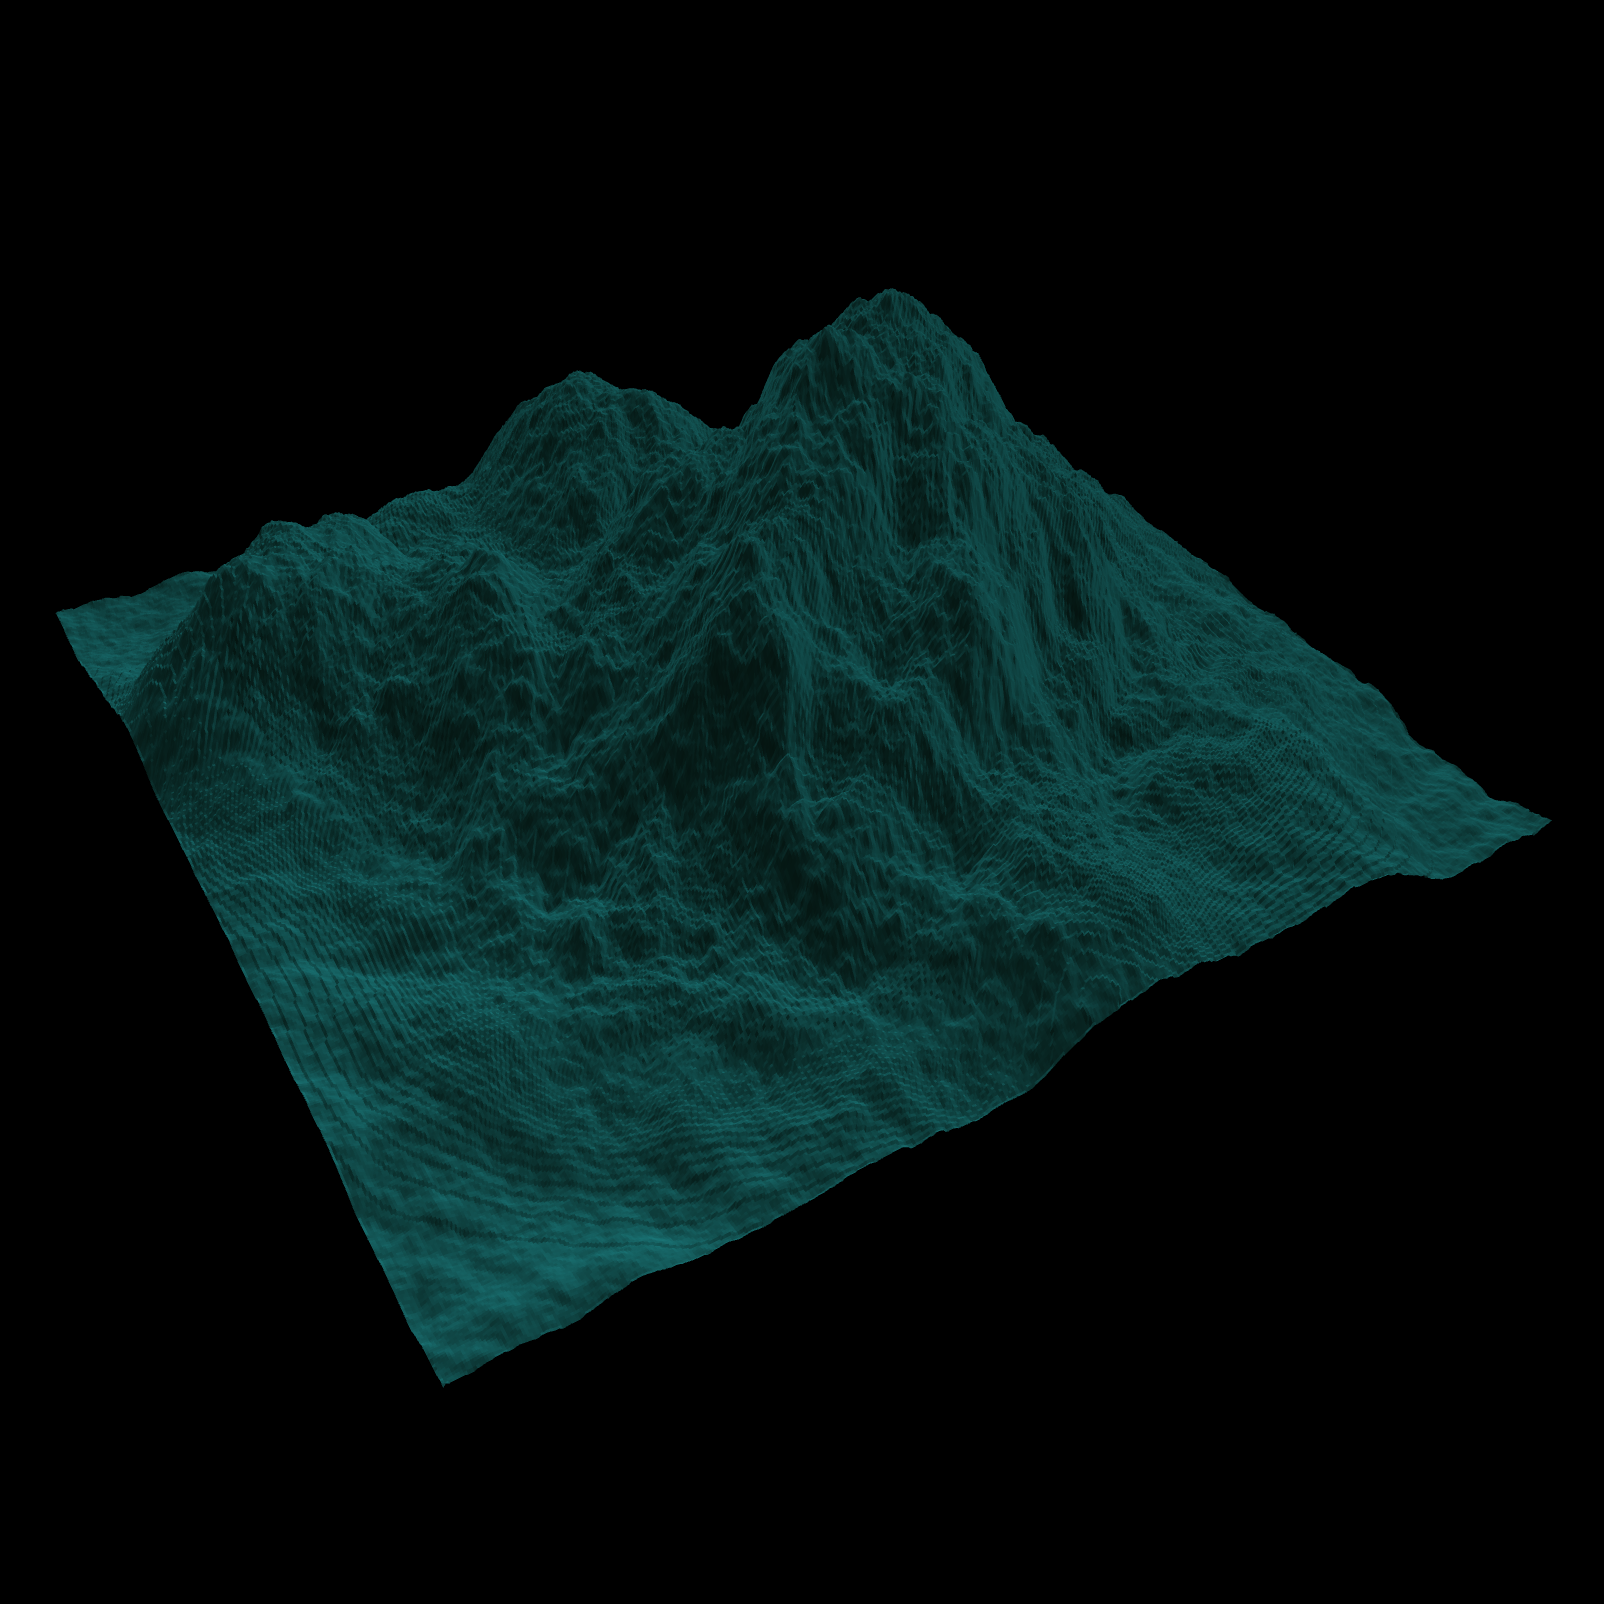
\includegraphics[width=\imagewidth]{images/results/terrains/512-1/fourier/20_3d}
		  \caption{$\beta = 2.0$}
		  \label{fig:ex-fourier20-surface}
		\end{figure}
		
		\begin{figure}[H]
		  \centering
		  
\includegraphics[width=\imagewidth]{images/results/terrains/512-1/fourier/22}
		  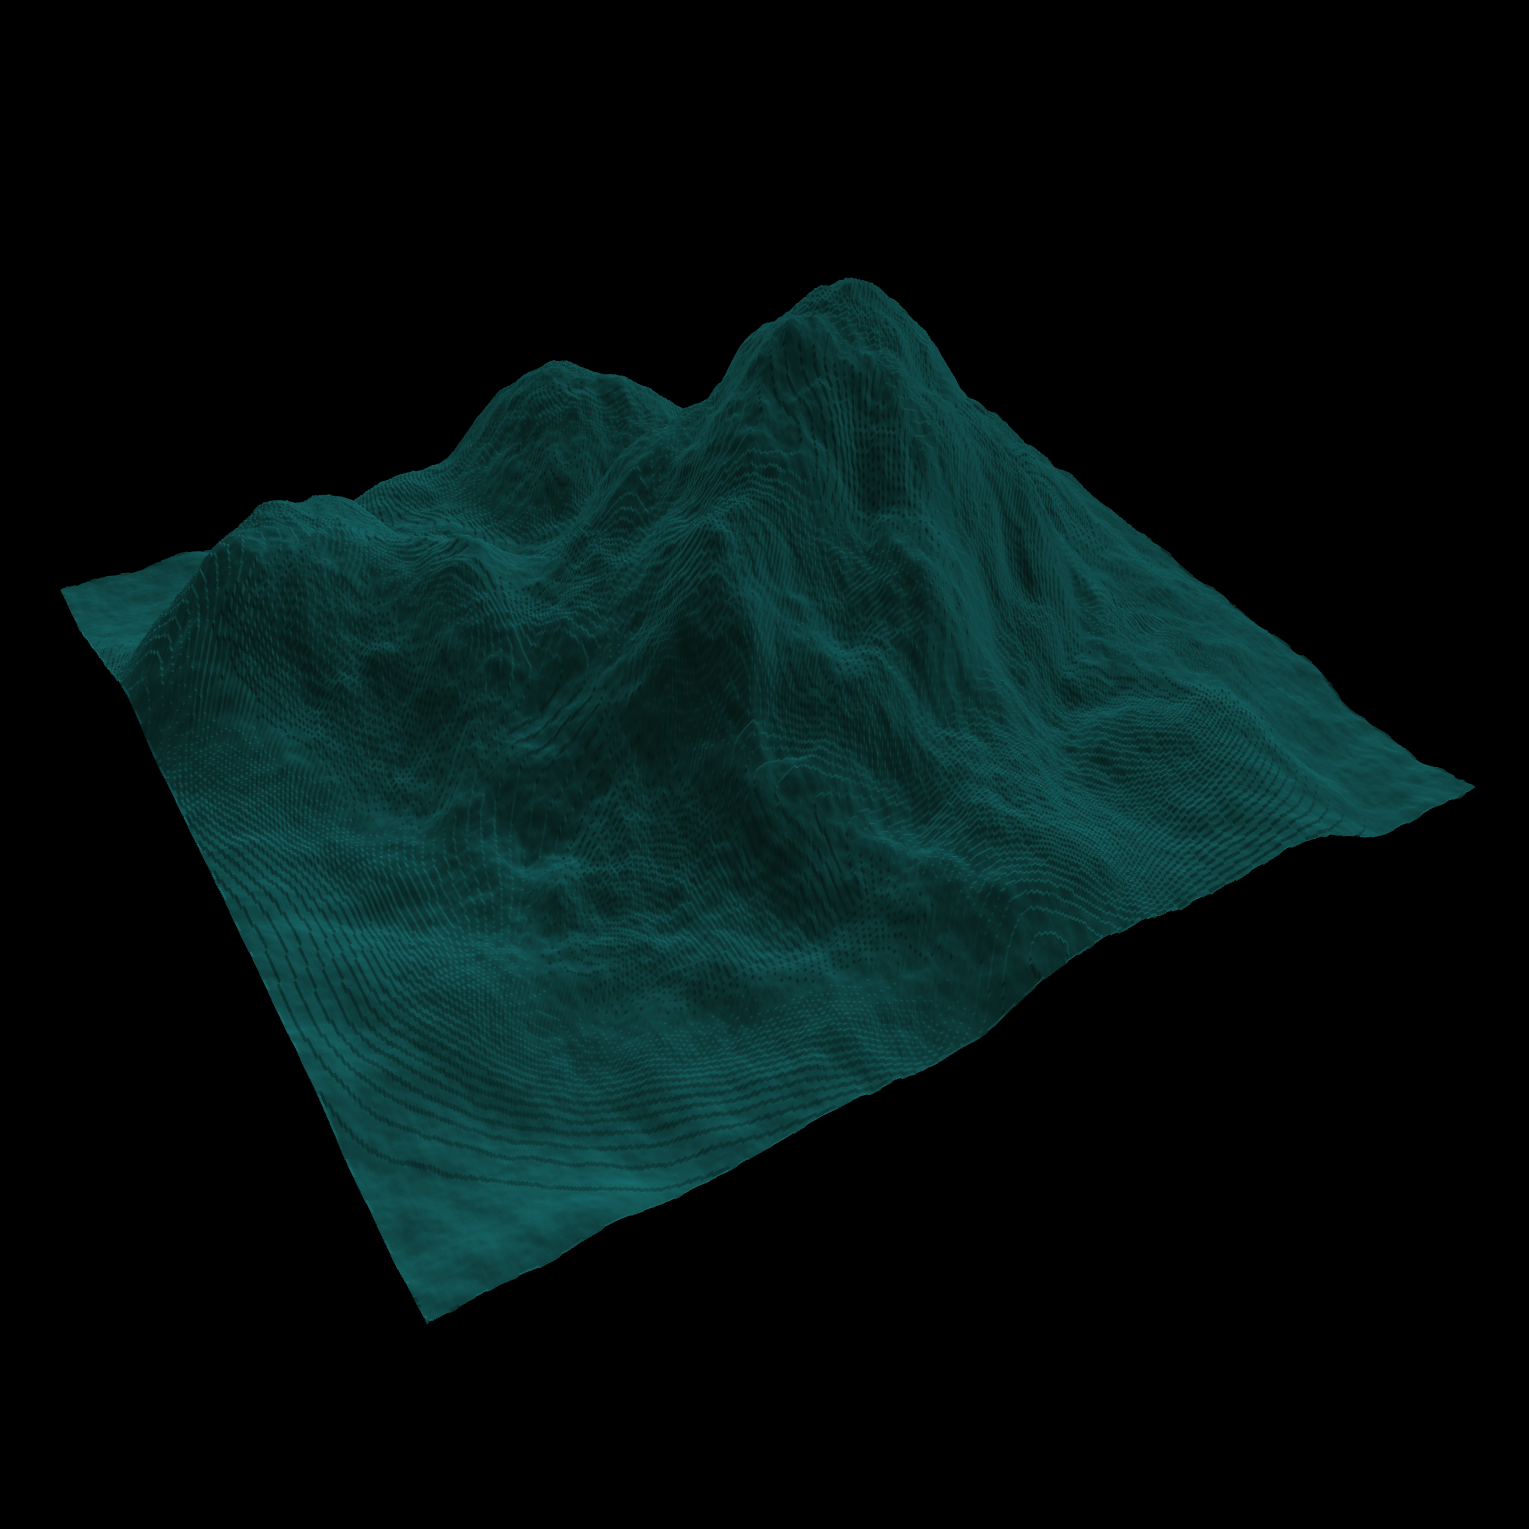
\includegraphics[width=\imagewidth]{images/results/terrains/512-1/fourier/22_3d}
		  \caption{$\beta = 2.2$}
		  \label{fig:ex-fourier22-surface}
		\end{figure}
		
		\begin{figure}[H]
		  \centering
		  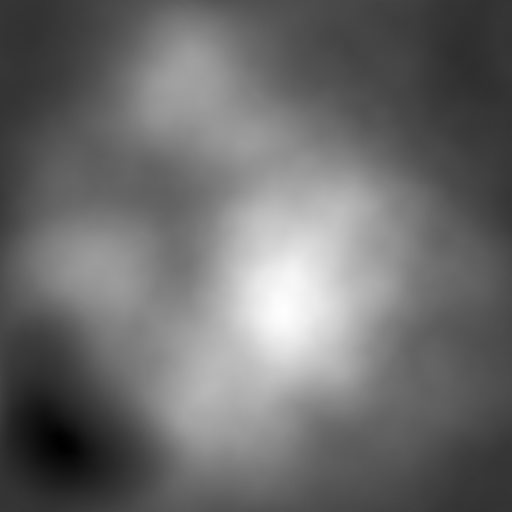
\includegraphics[width=\imagewidth]{images/results/terrains/512-1/fourier/24}
		  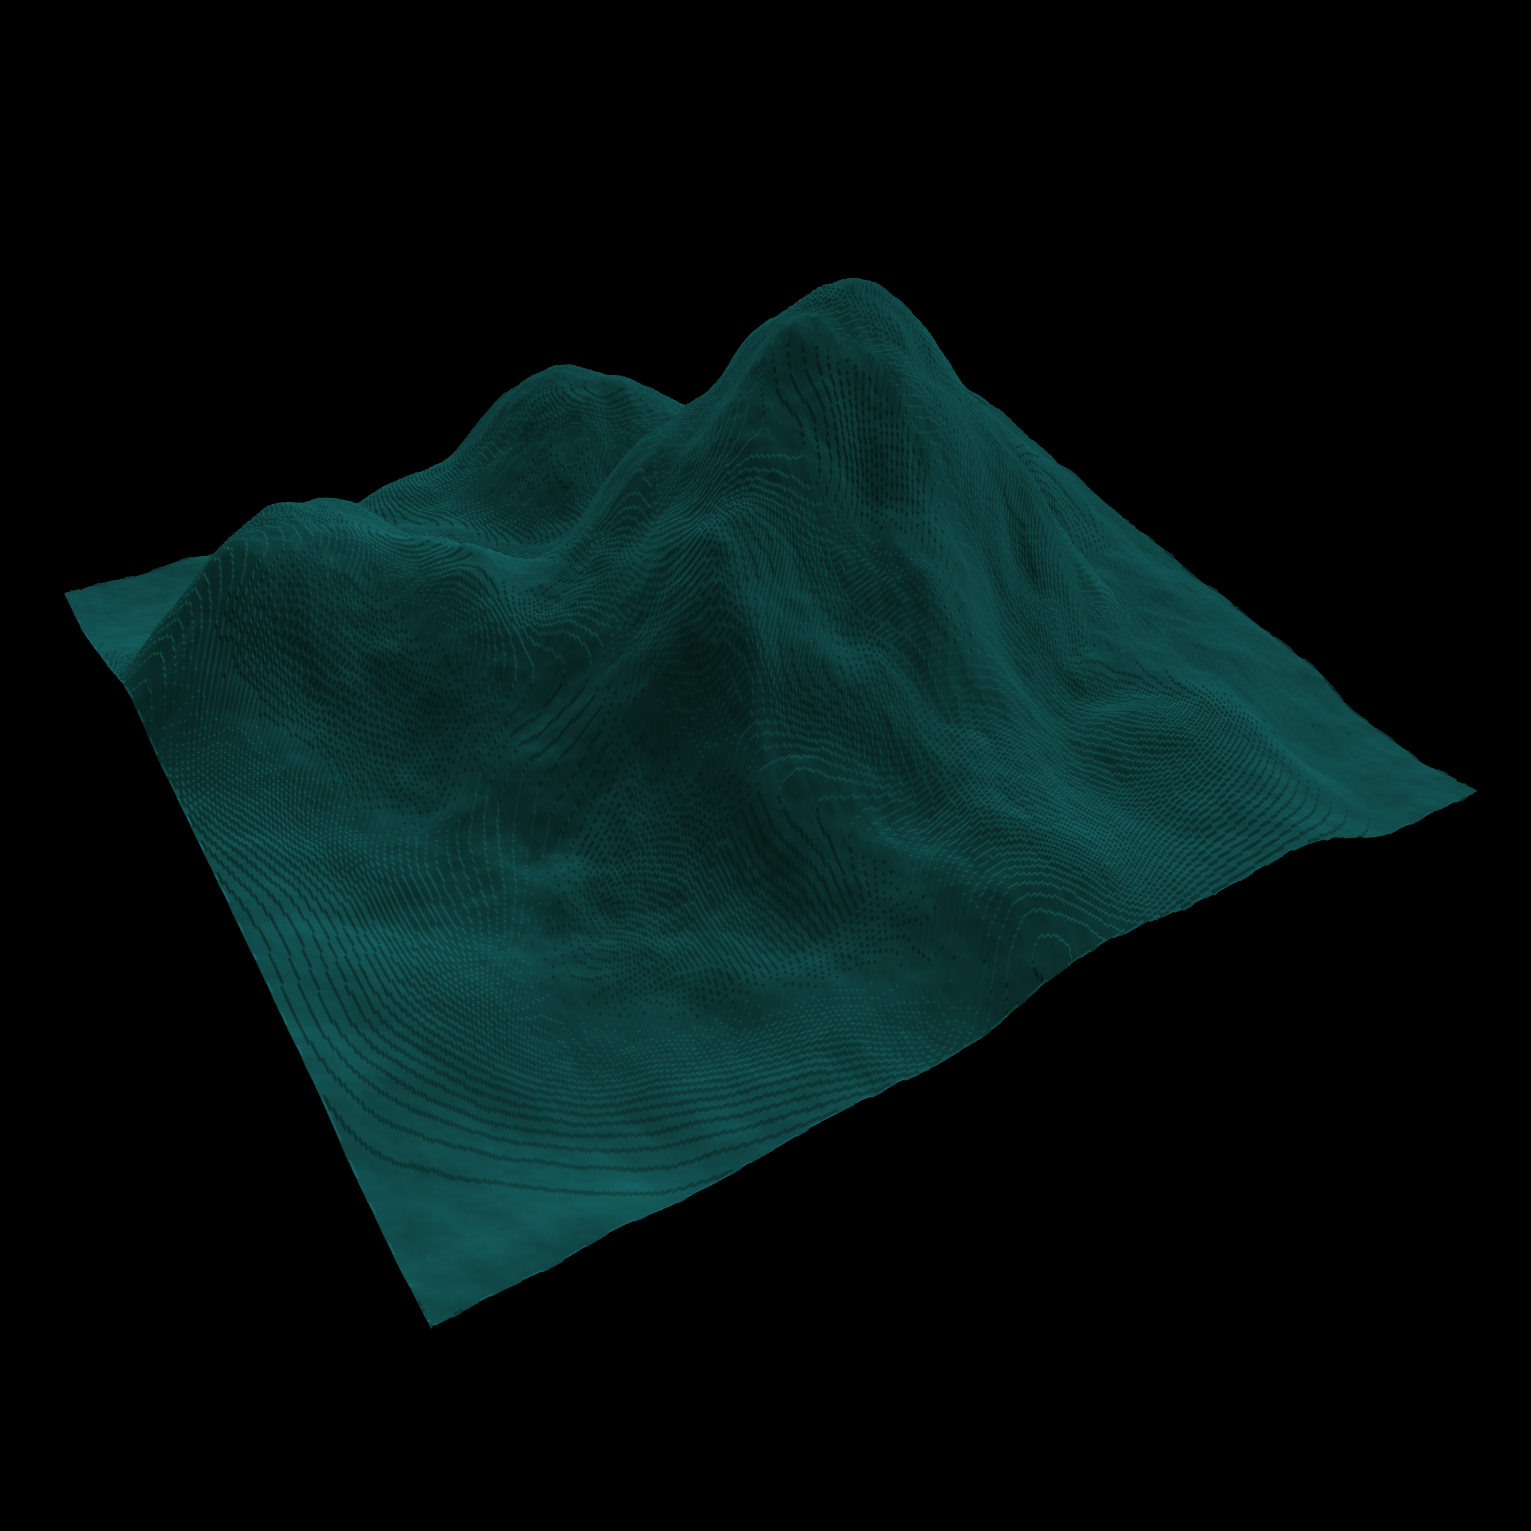
\includegraphics[width=\imagewidth]{images/results/terrains/512-1/fourier/24_3d}
		  \caption{$\beta = 2.4$}
		  \label{fig:ex-fourier24-surface}
		\end{figure}
		
    \subsection{Noise Synthesis}
      
      \subsubsection{Perlin Noise}
      
   		\begin{figure}[H]
  			\centering
  			
\includegraphics[width=\imagewidth]{images/results/terrains/512-1/perlin/120}
  			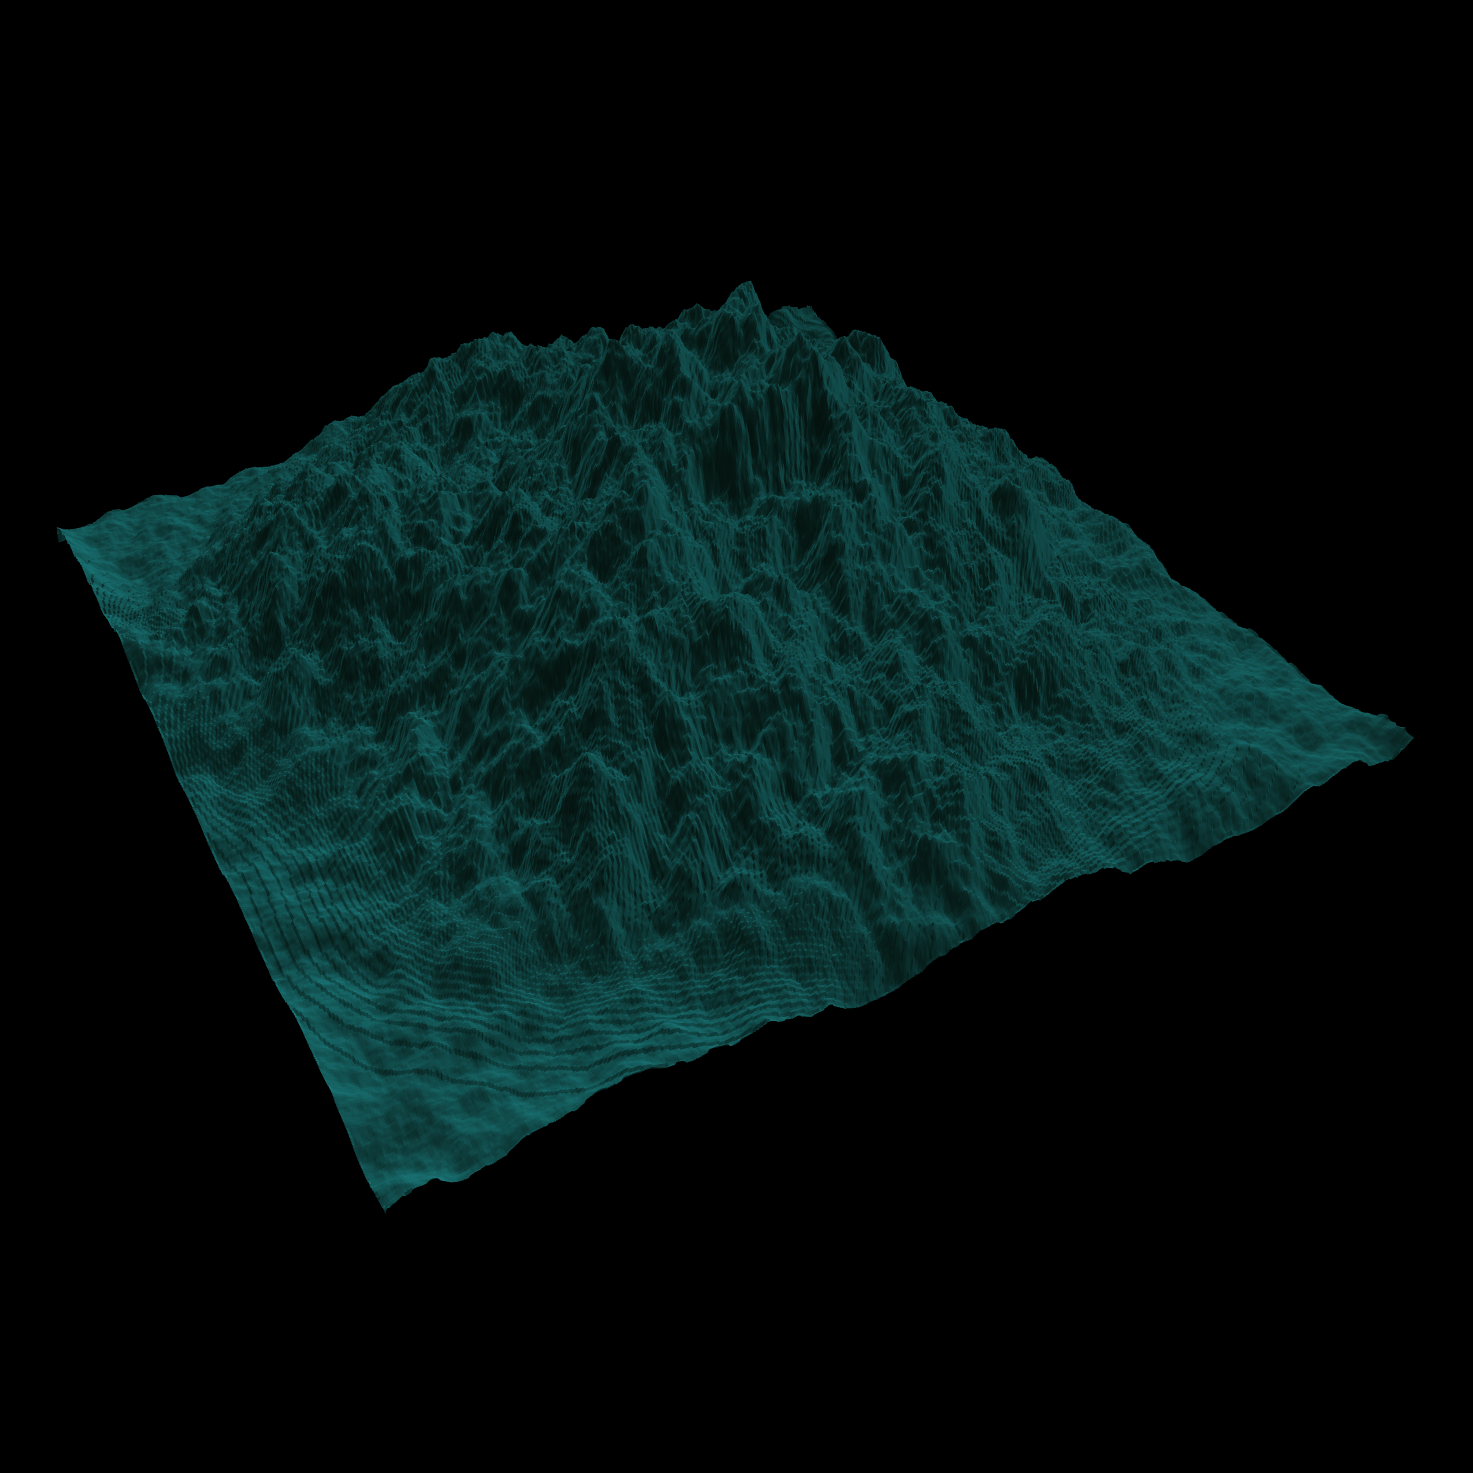
\includegraphics[width=\imagewidth]{images/results/terrains/512-1/perlin/120_3d}
  			\caption{$frequency = 120$}
  			\label{fig:ex-perlin120-surface}
   		\end{figure}
   		
   		\begin{figure}[H]
   			\centering
   			
\includegraphics[width=\imagewidth]{images/results/terrains/512-1/perlin/240}
   			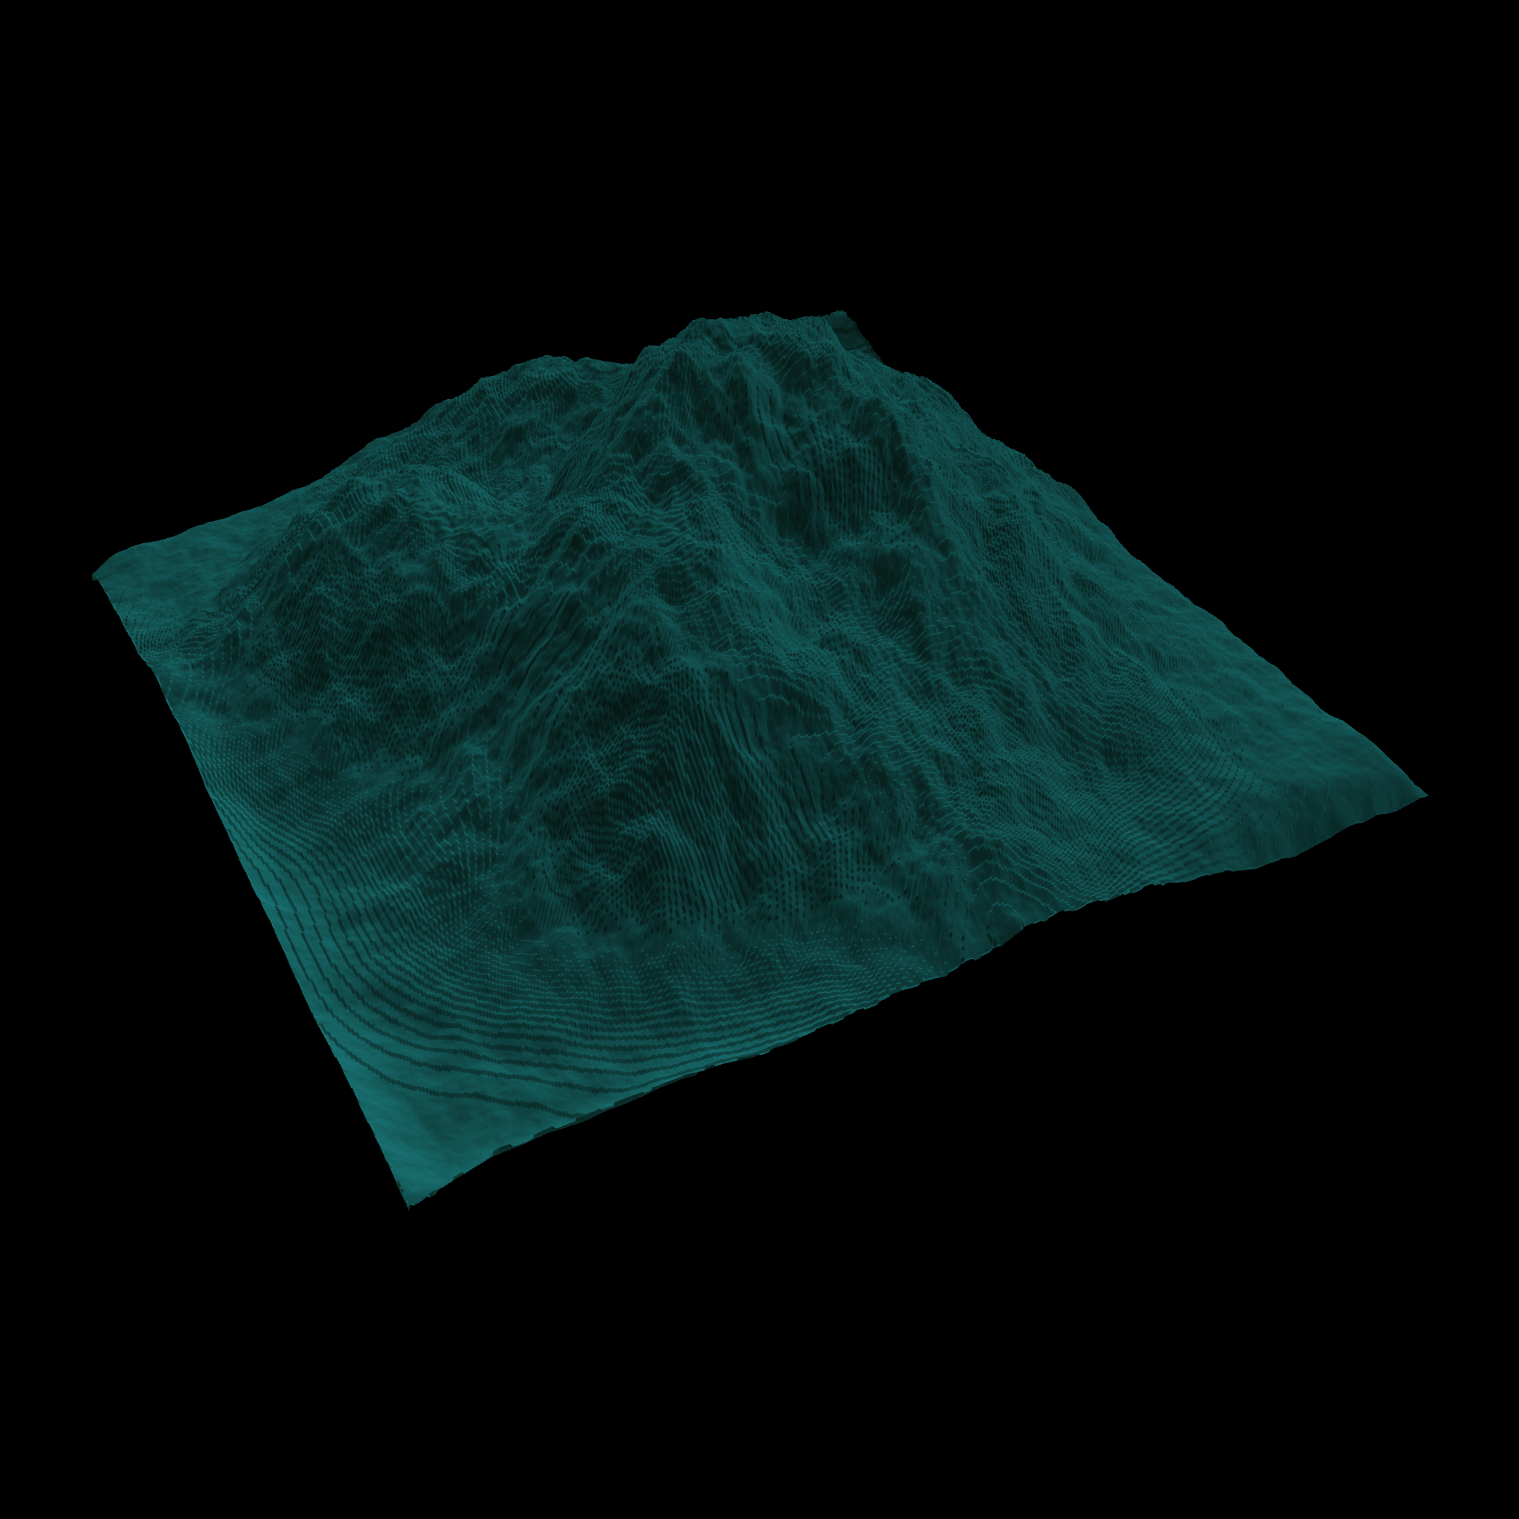
\includegraphics[width=\imagewidth]{images/results/terrains/512-1/perlin/240_3d}
  			\caption{$frequency = 240$}
   			\label{fig:ex-perlin240-surface}
   		\end{figure}
   		
   		\begin{figure}[H]
   			\centering
   			
\includegraphics[width=\imagewidth]{images/results/terrains/512-1/perlin/360}
   			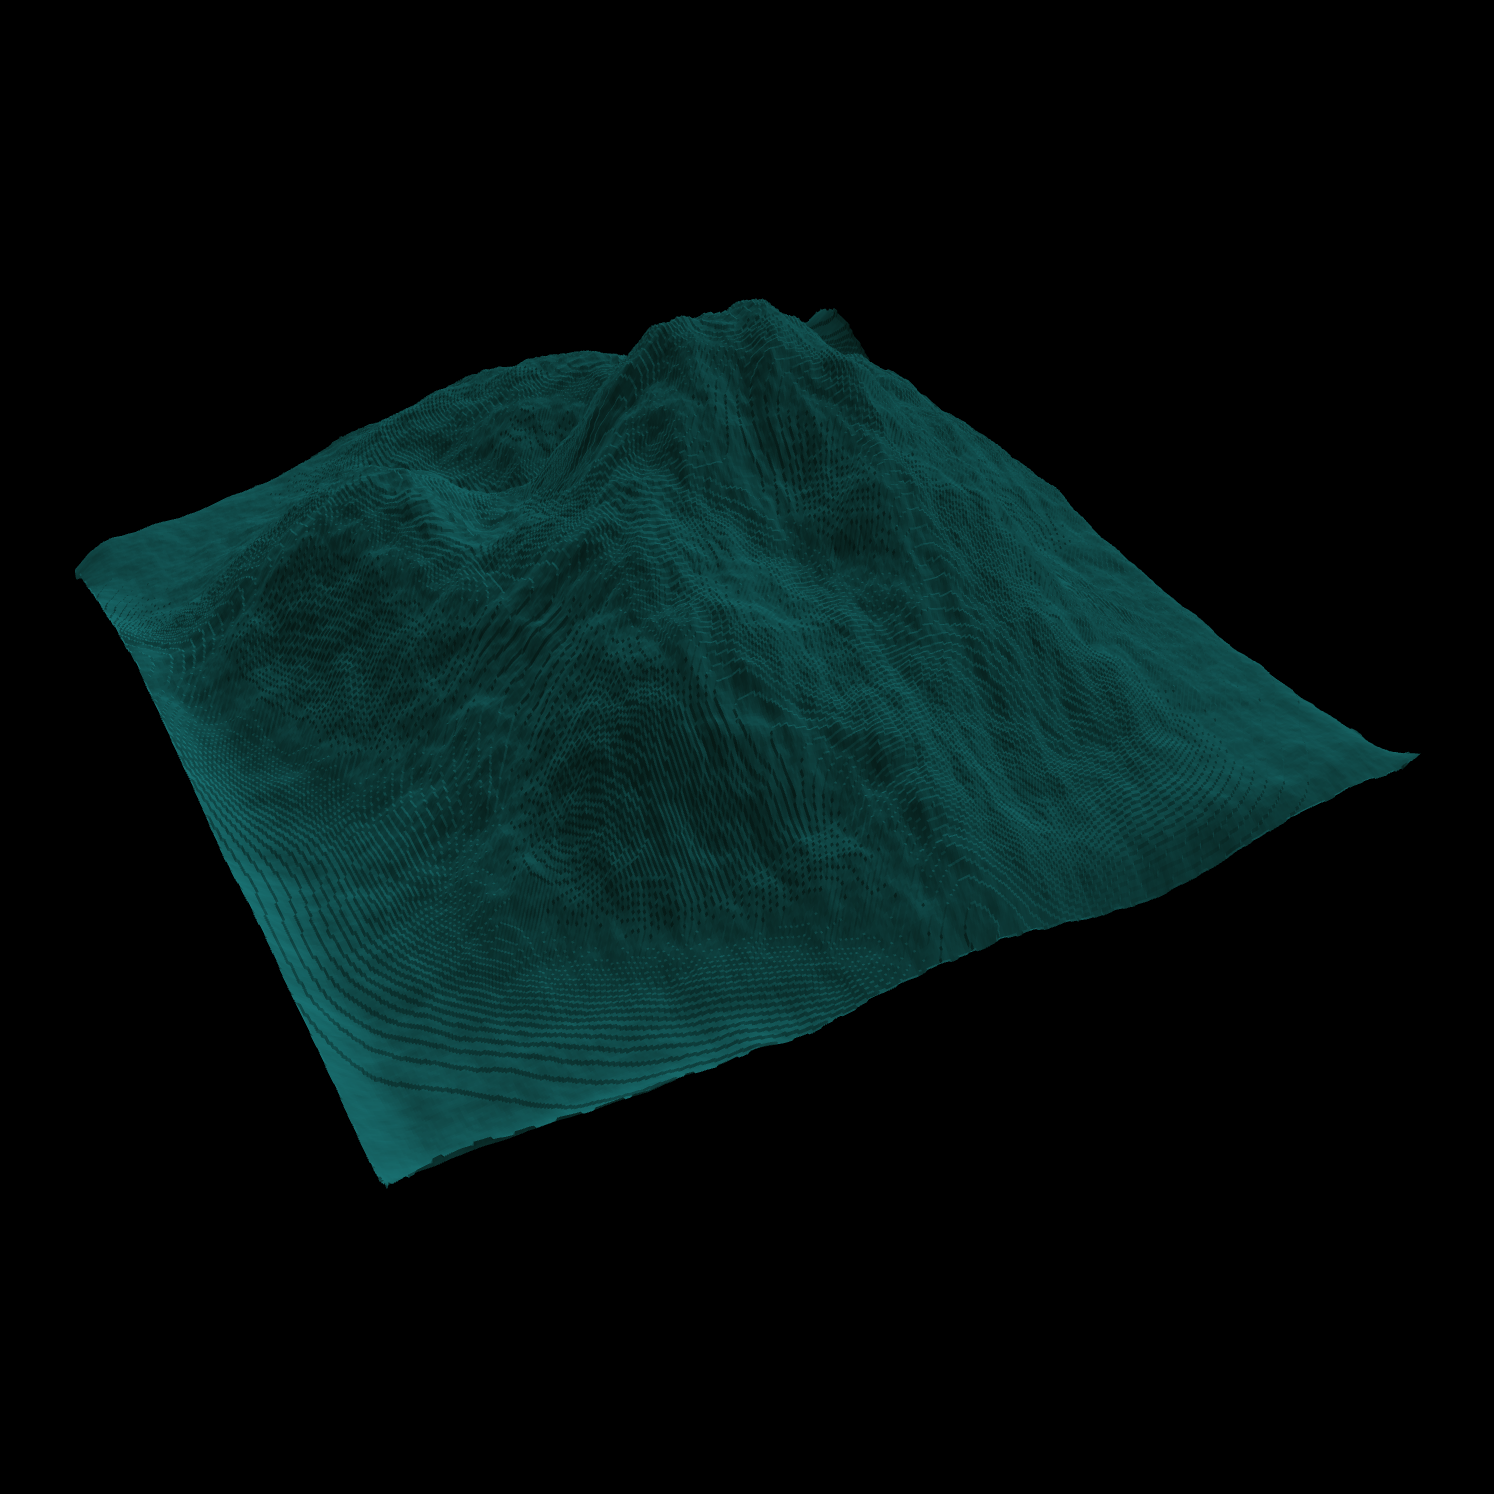
\includegraphics[width=\imagewidth]{images/results/terrains/512-1/perlin/360_3d}
  			\caption{$frequency = 360$}
   			\label{fig:ex-perlin360-surface}
   		\end{figure}
   		
   		\begin{figure}[H]
   			\centering
   			
\includegraphics[width=\imagewidth]{images/results/terrains/512-1/perlin/480}
   			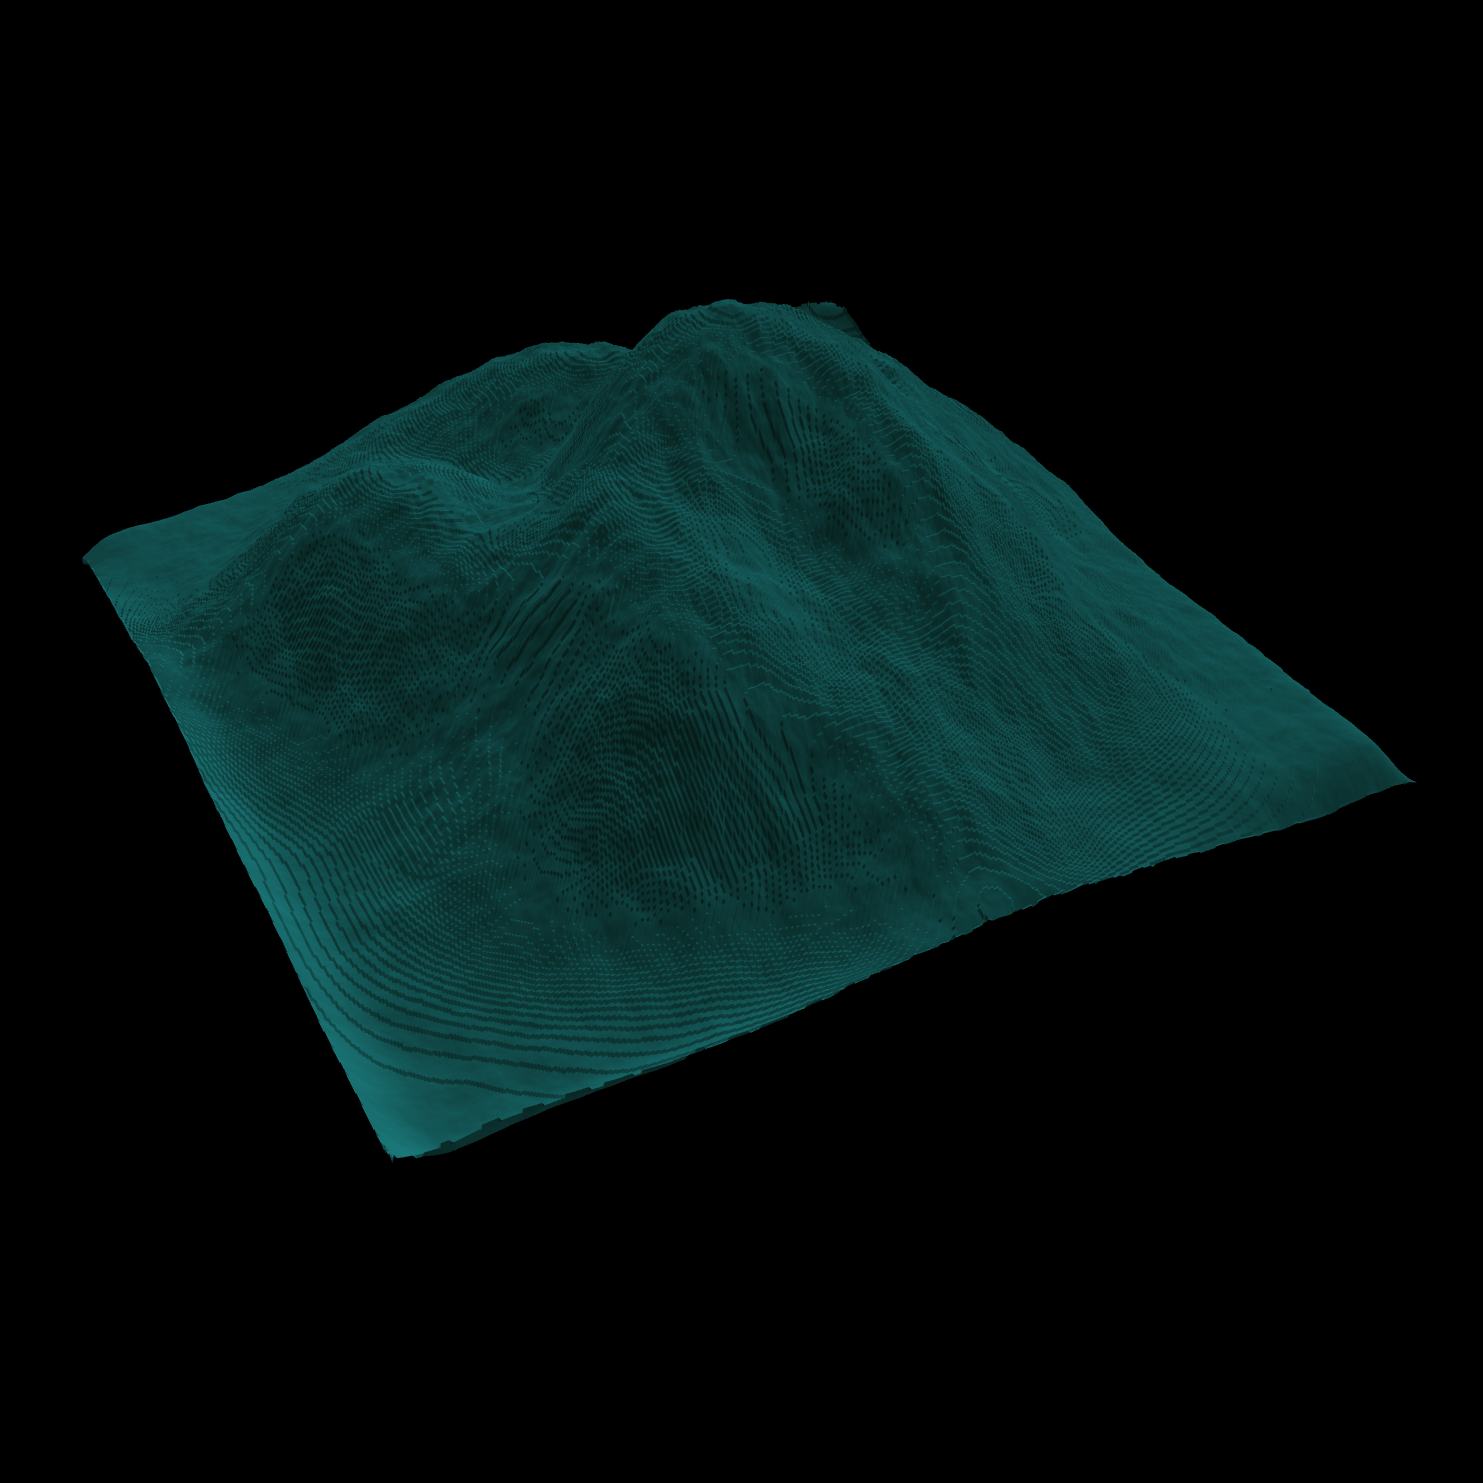
\includegraphics[width=\imagewidth]{images/results/terrains/512-1/perlin/480_3d}
  			\caption{$frequency = 480$}
   			\label{fig:ex-perlin480-surface}
   		\end{figure}
    
    
  
  \section{Random Generation Methods Performance}

    \begin{figure}[H]
    	\centering
    	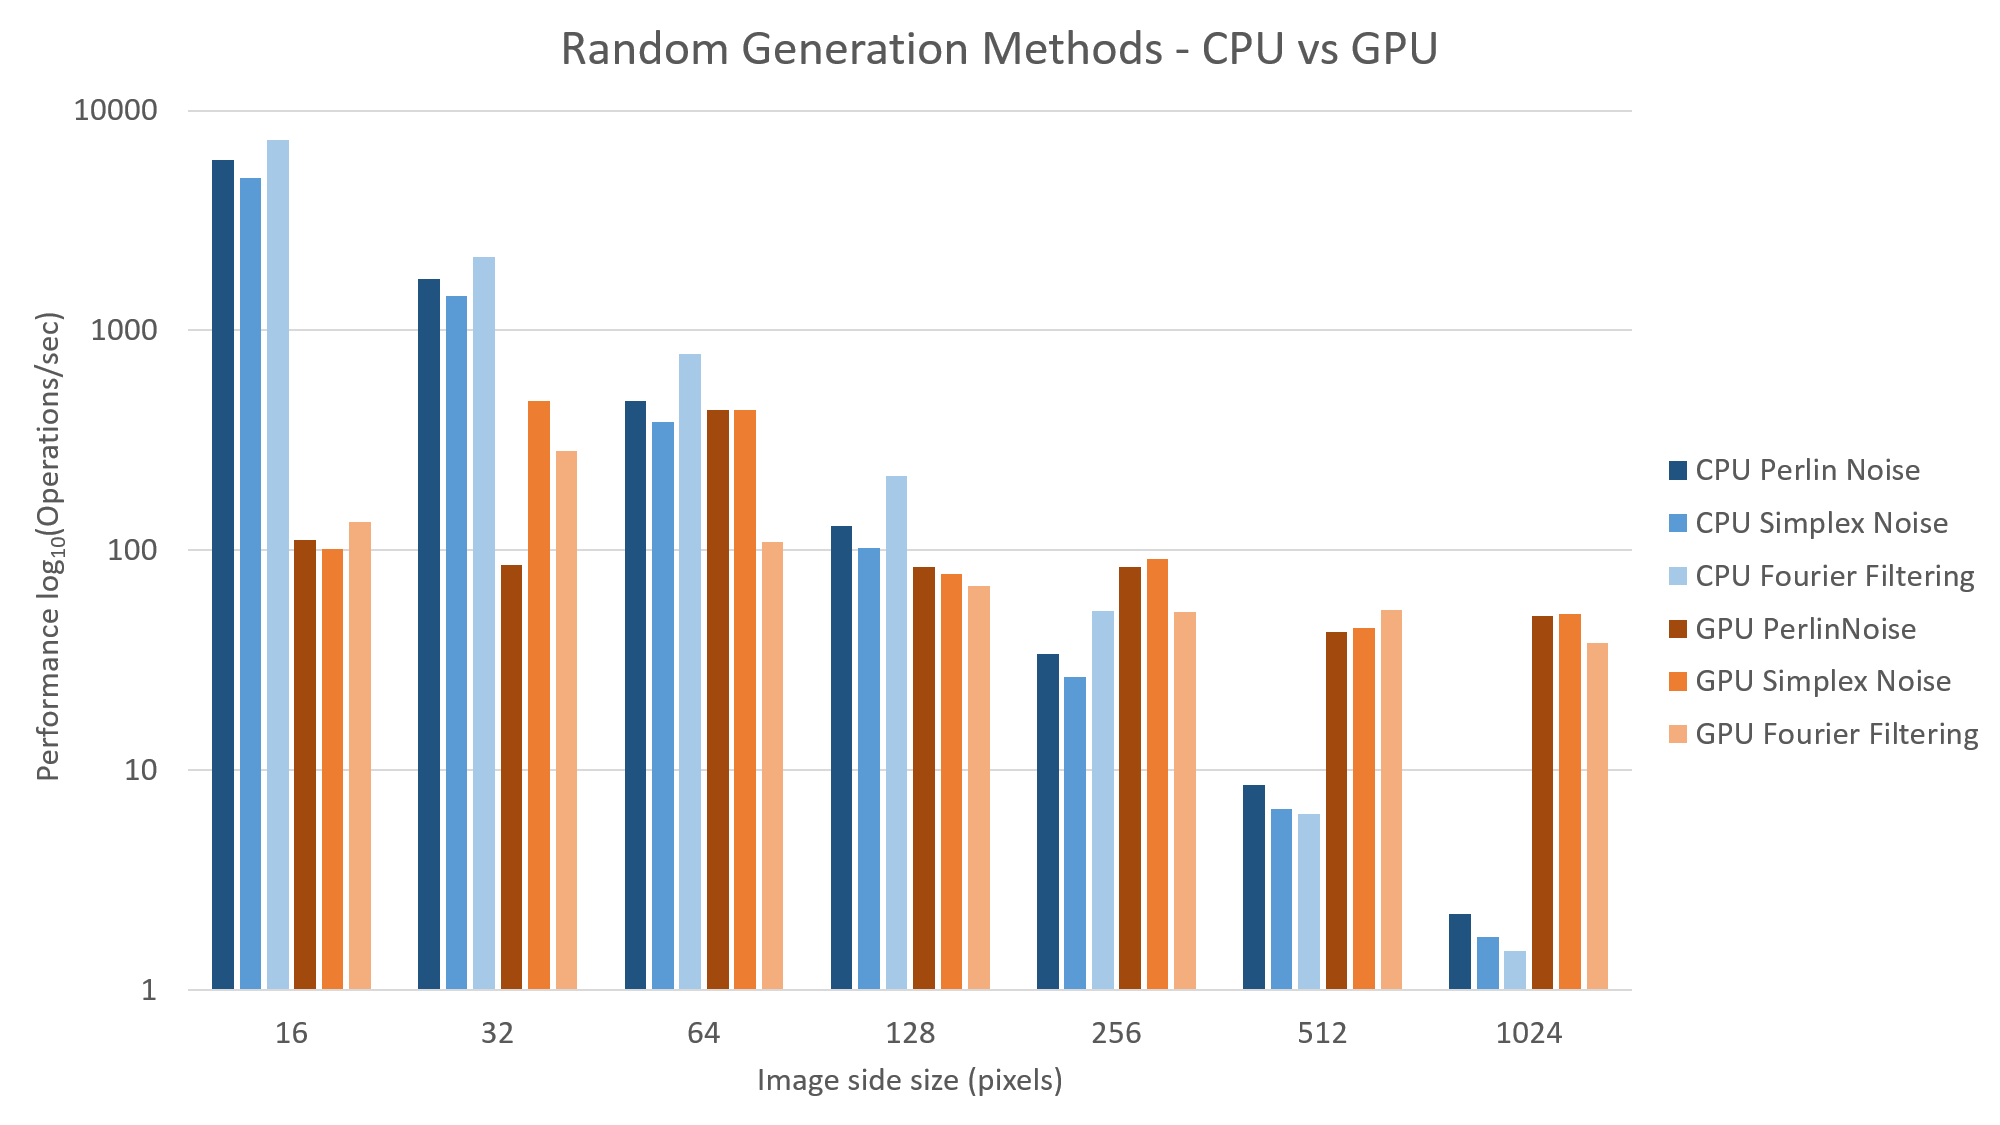
\includegraphics[width=\plotwidth]{images/results/benchmarks/plot-rgm}
    	\caption{Random Generation Methods Performance}
    	\label{fig:plot-rgm}
    \end{figure}
    
    With the objective of evaluating the performance from the random generation methods, both when executed in the CPU and in the GPU, some benchmarks were performed. The results from these tests are shown in Figure \ref{fig:plot-rgm} \review{where it can be seen that when the generation size is greater or equal to 256 the GPU implementation is faster. Additionally it is also possible to note that the noise synthesis methods execute faster than the fourier filtering.}
  
  \section {GPU vs CPU Computations Benchmarks}
    
    \begin{notes}
      \item Should I talk about the big-O for each solution?
    \end{notes}
    
    In order to evaluate the GPU Computations' performance some benchmarks were implemented and executed. In these benchmarks, the number of operations per second of the GPU implementation is compared with a reference CPU implementation. To be noted that all the measures assume that the required parameters are already in the testing device and the result is to remain in the same device, that is, the upload/download time is not measured. Additionally, due to the lazy initialization of the GPU computations framework, all the operations are initialized before the tests are run. 
    
    All the computations were performed using an Intel\textsuperscript{\textregistered} Core\textsuperscript{\texttrademark} i7-6700HQ CPU with 16 GB of RAM, with a NVIDIA\textsuperscript{\textregistered} GeForce\textsuperscript{\textregistered} GTX 950M GPU with 2 GB of VRAM, running Microsoft\textsuperscript{\textregistered} Windows\textsuperscript{\textregistered} 10 build 10586 64 bits, NVIDIA Driver version 365.10 and Google Chrome Version 51\footnote{Additionally Google Chrome had the flags \textit{\#enable-webgl-draft-extensions} and \textit{\#enable-unsafe-es3-apis} active in order for WebGL 2.0 to be available.}.
    
    \subsection{Fast Fourier Transform Benchmark}
    
      This test measures the performance of computing a Fast Fourier Transform. The results of this benchmark are shown in Figure \ref{fig:plot-fft}, where for each size of a square matrix the base 10 logarithm of the number of operations per second is plotted, \review{from which it can be seen that for square matrices of size up to 32 pixels, the CPU implementation is faster, while for larger matrices the GPU implementation prevails.}
    
      \begin{figure}[H]
      	\centering
      	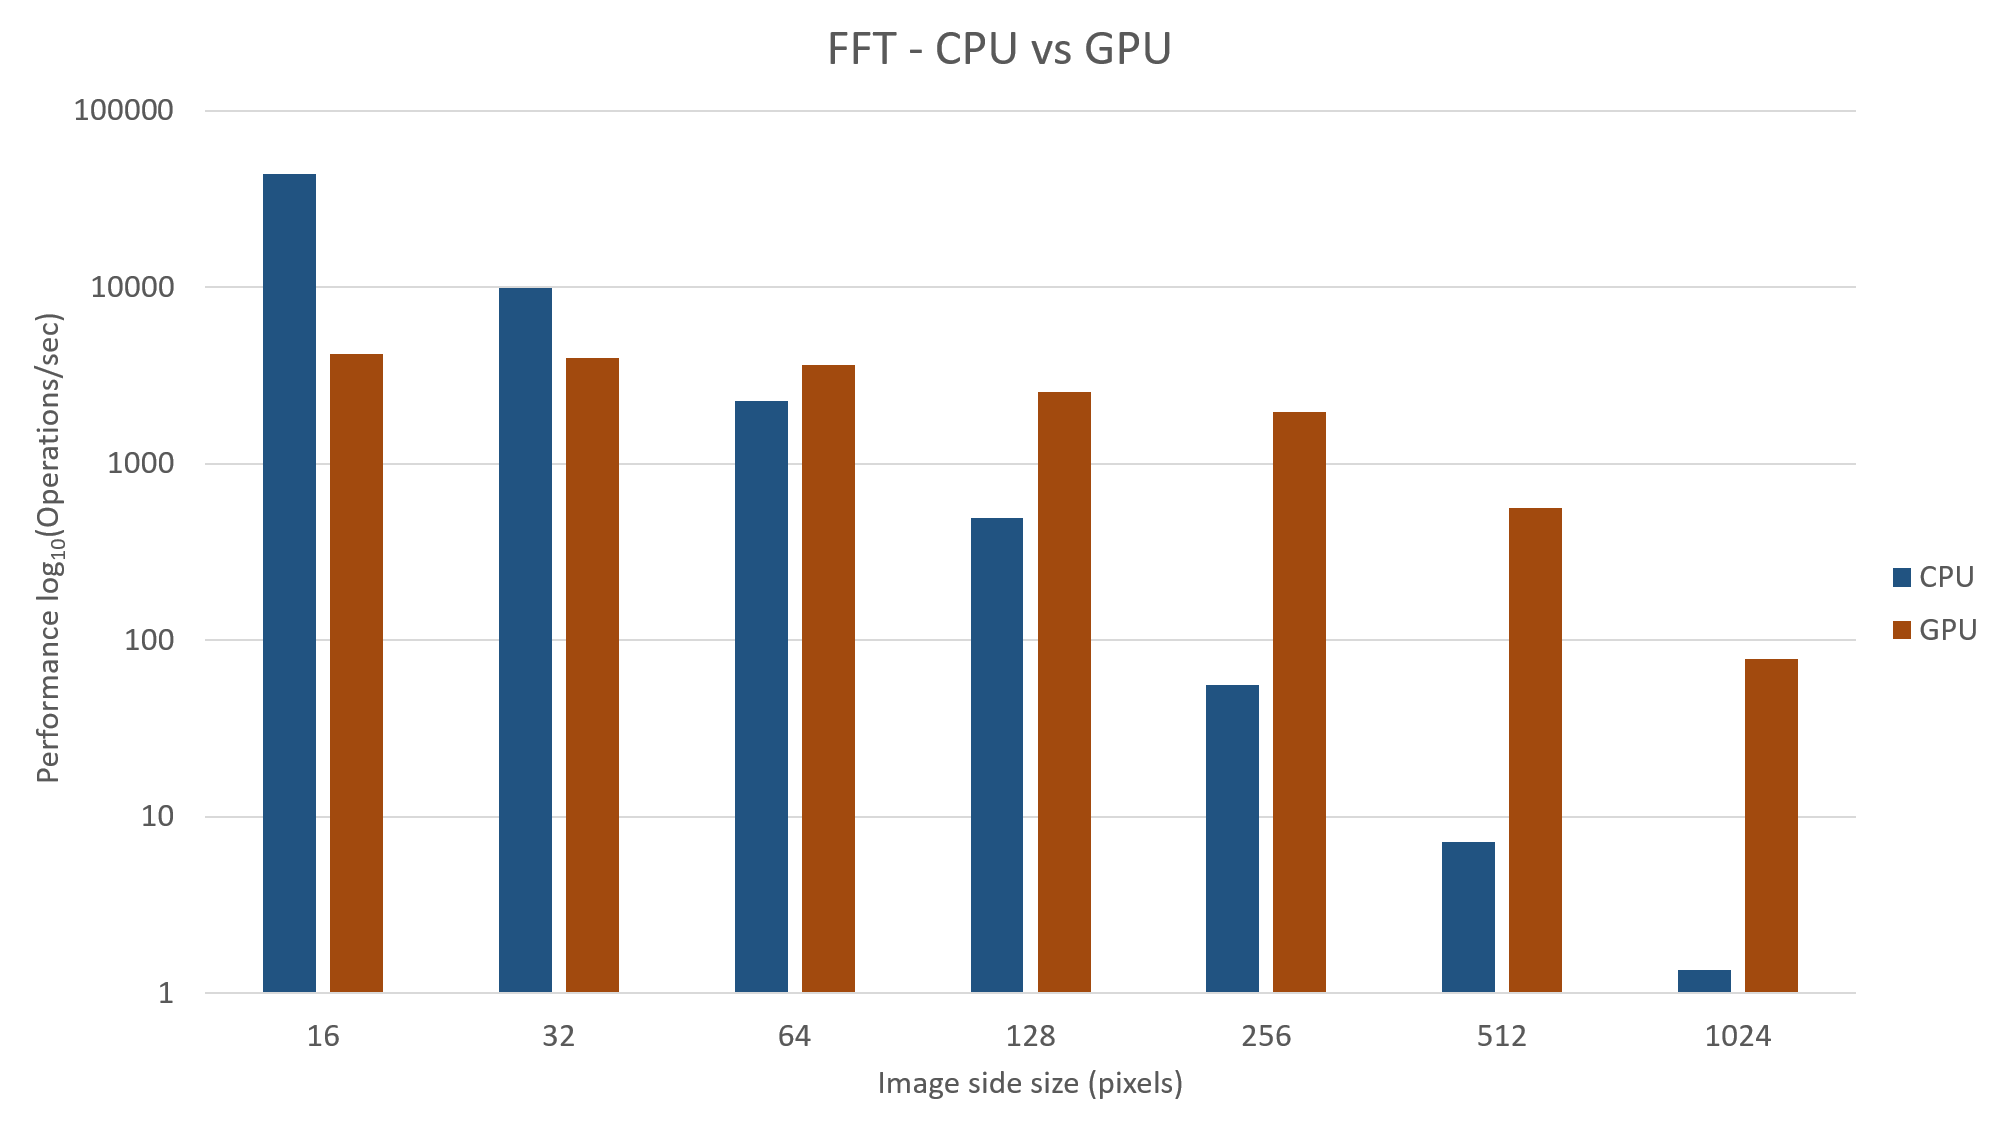
\includegraphics[width=\plotwidth]{images/results/benchmarks/plot-fft}
      	\caption{FFT benchmarks GPU vs CPU comparison}
      	\label{fig:plot-fft}
      \end{figure}
      
    \subsection{Element-wise Operations Benchmark}
    
      This test measures the performance of the element-wise operations: addition, subtraction and multiplication, when applied to two matrices. The results obtained from these computations can be seen in Figure \ref{fig:plot-ewops}, where a plot is shown mapping each size of a square matrix to the base 10 logarithm of the number of operations per second. \review{It can be noted that for square matrices up to 64 pixels the CPU operations are faster or perform the same as their GPU counterparts, while for bigger matrices the GPU implementation is better. Additionally it can also be seen that, in the CPU implementation, the addition operation is faster than the subtraction and multiplication operations.}
    
      \begin{figure}[H]
      	\centering
      	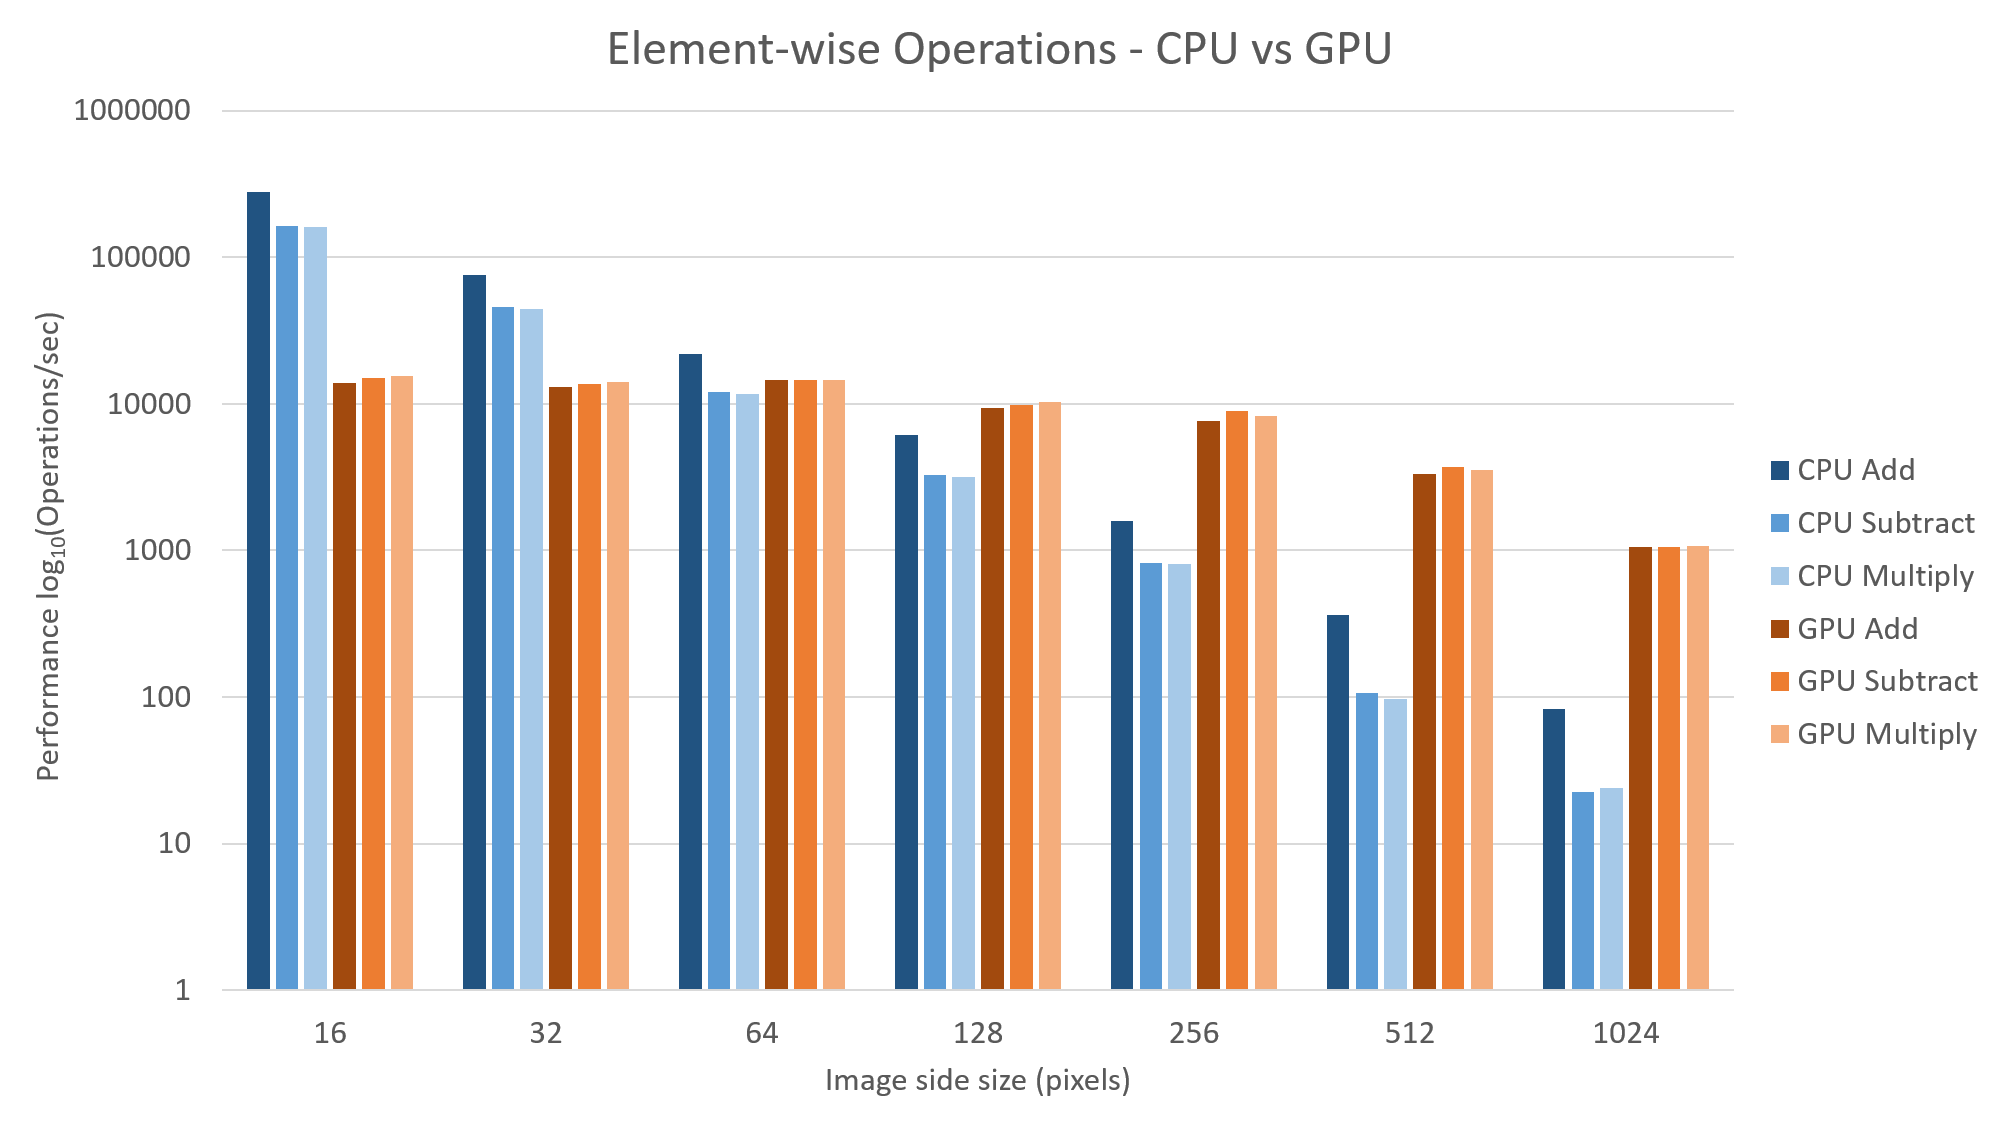
\includegraphics[width=\plotwidth]{images/results/benchmarks/plot-ewops}
      	\caption{Element-wise operations benchmarks GPU vs CPU comparison}
      	\label{fig:plot-ewops}
      \end{figure}
    
    \subsection{Normalization Benchmark}
    
      This benchmark aims to measure the performance of the normalization operation. In Figure \ref{fig:plot-normalization} a plot representing the results in logarithmic scale is shown. \review{From this plot it can be seen that the GPU implementation surpasses the CPU for square matrices with size 512 or 1024, while the CPU implementation is faster for smaller matrices.}
    
      \begin{figure}[H]
      	\centering
      	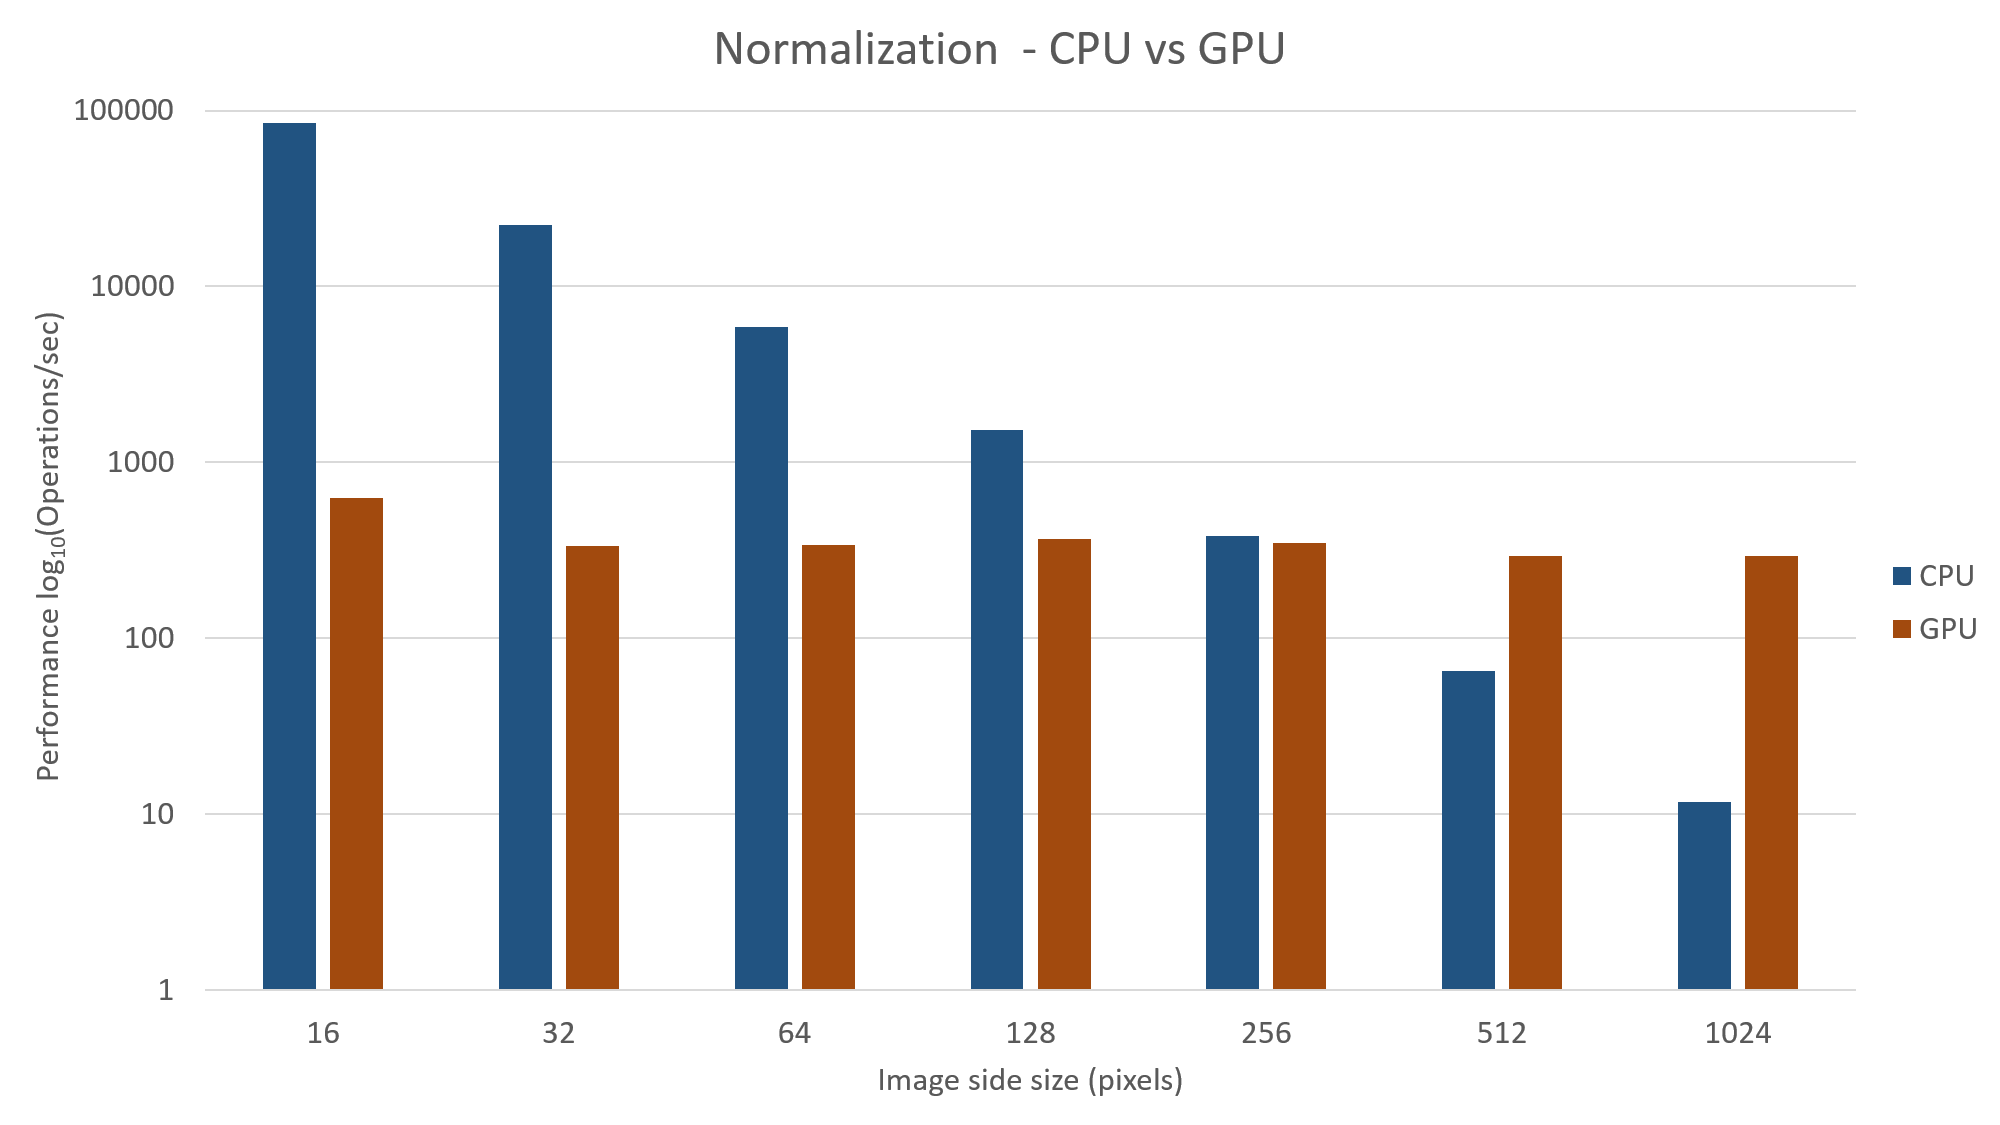
\includegraphics[width=\plotwidth]{images/results/benchmarks/plot-normalization}
      	\caption{Normalization benchmarks GPU vs CPU comparison}
      	\label{fig:plot-normalization}
      \end{figure}
    
    \subsection{Benchmark Summary}
    
      \review{In summary, for square matrices with size greater or equal to 256 the GPU implementations perform better than it's CPU counterparts. This fact can be noted in Figure \ref{fig:plot-ratios} where the ratio of the GPU over the CPU performances is shown, in base 10 logarithmic scale, for each size and for each benchmark executed.}
    
      \begin{figure}[H]
      	\centering
      	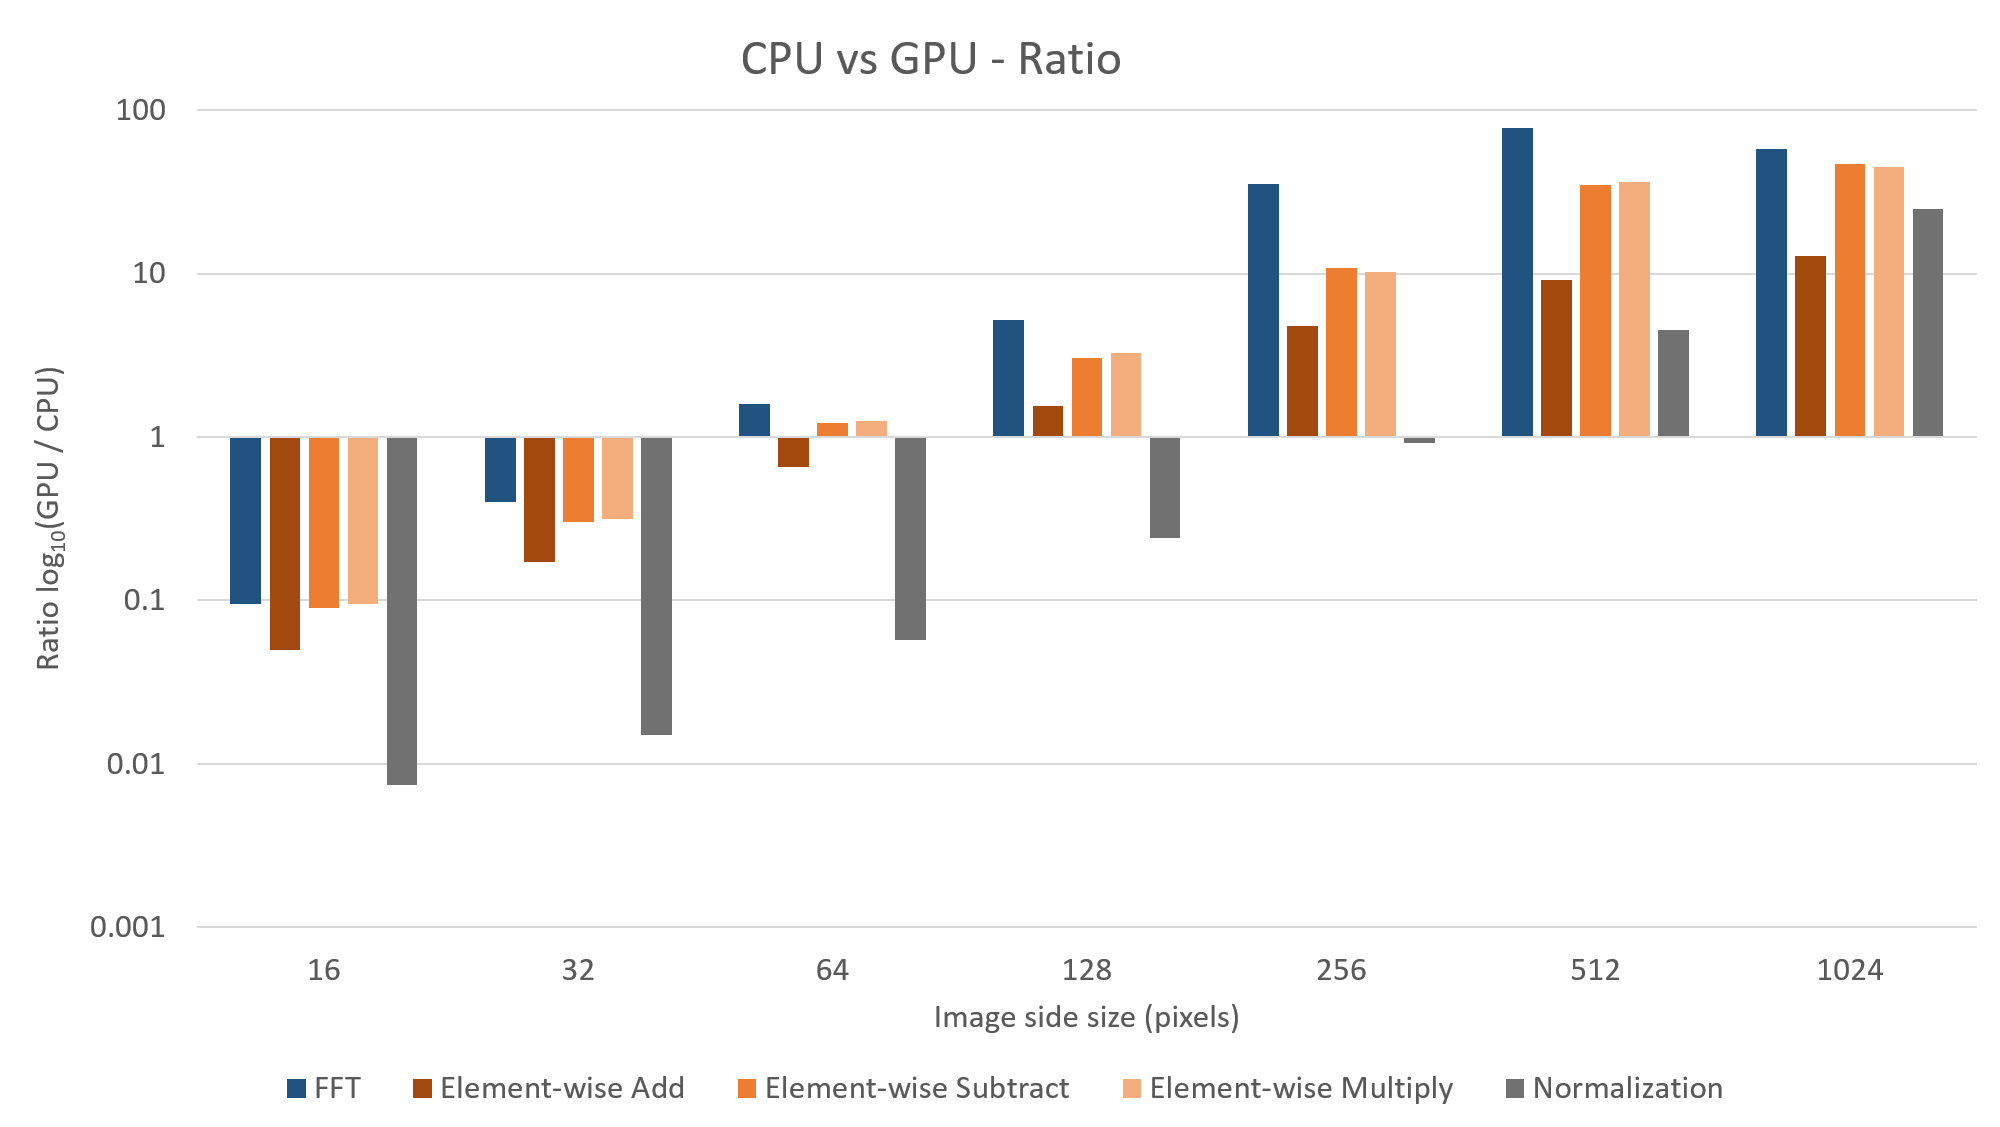
\includegraphics[width=\plotwidth]{images/results/benchmarks/plot-ratios}
      	\caption{GPU vs CPU ratios}
      	\label{fig:plot-ratios}
      \end{figure}
      